\documentclass[11pt]{article}

% ============================================================
%  claudeFinal.tex
%  Electroweak Mass Ratios from an Internal SU(2):
%  A Kaluza-Klein Reading of the de Vries Relation
%
%  A self-contained, Witten-style theoretical essay.
%  Single-column preprint format, suitable for Physical Review D.
% ============================================================

\usepackage[a4paper,margin=1in]{geometry}
\usepackage{amsmath,amssymb,amsthm}
\usepackage{mathtools}
\usepackage{slashed}
\usepackage{bm}
\usepackage{booktabs}
\usepackage{longtable}
\usepackage{graphicx}
\usepackage{tikz}
\usepackage{pgfplots}
\pgfplotsset{compat=1.18}
\usetikzlibrary{arrows.meta,positioning,calc,decorations.pathmorphing}
\usepackage[hidelinks]{hyperref}

% ---- theorem environments -------------------------------------------------
\theoremstyle{plain}
\newtheorem{theorem}{Theorem}[section]
\newtheorem{proposition}[theorem]{Proposition}
\newtheorem{lemma}[theorem]{Lemma}
\newtheorem{corollary}[theorem]{Corollary}
\theoremstyle{definition}
\newtheorem{axiom}{Axiom}
\newtheorem{remark}[theorem]{Remark}
\newtheorem{definition}[theorem]{Definition}

% ---- macros ---------------------------------------------------------------
\newcommand{\cA}{\mathcal{A}}
\newcommand{\cD}{\mathcal{D}}
\newcommand{\cH}{\mathcal{H}}
\newcommand{\cK}{\mathcal{K}}
\newcommand{\cL}{\mathcal{L}}
\newcommand{\cM}{\mathcal{M}}
\newcommand{\cO}{\mathcal{O}}
\newcommand{\Xp}{X_{+}}
\newcommand{\Xm}{X_{-}}
\newcommand{\half}{\tfrac12}
\newcommand{\threeq}{\tfrac34}
\newcommand{\sinsq}{\sin^{2}\theta_W}
\newcommand{\Tr}{\operatorname{Tr}}
\newcommand{\dd}{\mathrm{d}}
\newcommand{\R}{\mathbb{R}}
\newcommand{\C}{\mathbb{C}}
\newcommand{\Z}{\mathbb{Z}}
\newcommand{\SU}{\mathrm{SU}}
\newcommand{\U}{\mathrm{U}}
\newcommand{\SO}{\mathrm{SO}}
\newcommand{\Sp}{\mathrm{Spin}}
\newcommand{\AdS}{\mathrm{AdS}}

\title{\bf Electroweak Mass Ratios from an Internal $\SU(2)$:\\[2mm]
A Kaluza--Klein Reading of the de Vries Relation}

\author{Claude\\[1mm]
\small (preprint; the status of each claim --- theorem, derived, structural,
or conjectural --- is stated in the text)}

\date{25 May 2026}

\begin{document}
\maketitle

\begin{abstract}
\noindent
The on-shell electroweak mixing angle, $\sinsq=0.2231$, and the
mass ratio $M_W^2/M_Z^2$ are reproduced to a few parts in $10^{4}$ by a
single algebraic object with no continuous free parameter: the positive
eigenvalue of the $2\times2$ ``branch operator''
$\cA(J)=\bigl(\begin{smallmatrix}0&\sqrt J\\ \sqrt J&-J\end{smallmatrix}\bigr)$,
evaluated at the Casimir labels $J=j(j+1)$ of the spins $j=0,\half,1$.
This is the empirical regularity --- the \emph{de Vries relation} --- that
we take as the clue fixing the internal geometry. The central claim of the
paper is that the internal manifold we live on is essentially fixed by the
Standard Model gauge content: the ten-dimensional Type IIA geometry
$M_4\times K_6$ with $K_6=\mathbb{CP}^2\times\mathbb{CP}^1$ --- the minimal
product of the minimal $\SU(3)$ coset (colour, four-dimensional) and the
minimal $\SU(2)$ coset (weak isospin, two-dimensional), saturating the
internal dimension $4+2=6$. (We are careful with ``unique'': this is the
minimal product realization, not a proven-unique manifold; see
Section~\ref{sec:k6}.)
We show that $\cA(J)$ is the linearized flux-fluctuation spectrum on this
$K_6$, and that its single scale modulus is what grows a seventh
dimension (recovering the well-understood eleven-dimensional $M^{pqr}$ of the
1980s, here a mere limit) and shrinks a fifth (the nine-dimensional infrared
endpoint). Three statements organize the operator. First, a
short representation-theoretic argument shows that the labels $j=0,\half,1$
are exactly the half-integer fingerprint of an $\SU(2)$ (rather than
$\SO(3)$) internal geometry, and that $J=j(j+1)$ is one quarter of the
scalar Laplacian eigenvalue on the unit $S^3$. Second, the off-diagonal
$\sqrt J$ is the matrix element of a \emph{first-order}, self-adjoint,
$\SU(2)$-covariant operator --- concretely the curl $\star\dd$ on
co-exact one-forms, whose square is the Hodge Laplacian; this is why the
mixing is a square root of the Casimir and not the Casimir itself. Third,
the negative diagonal is the form-degree mixing induced by the
ten-dimensional Type IIA background flux on $K_6$, with a coefficient $c$
whose self-dual value $c=1$ gives the de Vries block. We prove a normal-form
theorem: a minimal set of axioms (gauge masslessness, Casimir factorization
of the mixing, a single generating operator, no free dimensionless constant)
forces $\cA(J)$ uniquely. We are careful not to overstate what this buys: the
weak angle is determined with no \emph{continuous} free parameter, but only
\emph{conditional} on the discrete inputs (the electroweak spin content
$j=\tfrac12,1$ and the coefficient $c=1$). For $c=1$ itself we give a
\emph{conditional derivation}: we prove that $c=1$ is forced if the order
parameter is a flat geometric modulus coupling to the flux through a single
Stückelberg portal (so the order-parameter mass is $-A_jA_j^\dagger$, built
from the same operator as the mixing), and that this $c=1$ is robust against
the Weitzenb\"ock curvature shift; we also show that the alternative ---
an independent, curvature-shifted order-parameter mass --- gives a
$j$-dependent $c=(4J+1)/(4J)$ and the wrong angle $0.267$, so the single-portal
condition does sharp, falsifiable work. The residual open problem is thereby
reduced from ``compute $c$'' to the specific statement that the electroweak
order parameter is a single-portal flat modulus; until it is established we
report, honestly, the one-parameter family $\sin^2\theta_W(c)$ with $c=1$
(on-shell $\sin^2\theta_W=0.2231$) as its structurally distinguished point,
and we apply to our own $c=1$ the same skepticism we apply to the classical
$M^{pqr}$ integer fit. We organize the whole
construction as a dimensional ladder $D=11\to D=10\to D=9$ read off by probe
energy and implemented by two distinct circle operations, and we argue that
the physical, chirality-bearing rung --- the one we live on --- is $D=10$:
chiral fermions are impossible from smooth eleven-dimensional reduction
(Witten's no-go) but arise from D-branes in the ten-dimensional Type IIA
interface, while the nine-dimensional infrared endpoint is chirality-trivial
because its residual $\SU(3)_c\times\U(1)_Q$ is vector-like. The de Vries
operator and the chiral fermions thus live on the same rung, $D=10$. We
identify the surviving $\U(1)_Q$ and the masslessness of the photon, and read
the electromagnetic coupling at the $D=9$ boundary. The negative branch of $\cA(J)$ is interpreted as the
electroweak order parameter and is shown to reproduce, with the same
single scale that fixes $M_W$ and $M_Z$, mass values near the Higgs and
top. We are explicit throughout about what is derived, what is a clean
structural consequence, and what remains a genuine dynamical assumption
--- the latter reducing to the \emph{single} statement that the flux
coefficient equals one. We close with a critical comparison to the
classical $M^{pqr}$ coupling-ratio program, explaining why a literal
integer-label fit to the weak angle is an over-determination of the data
rather than a prediction, and we list the parameter-free, near-term
falsifiable consequences of the construction, including a neutral
spin-zero state near $96.5\,$GeV.
\end{abstract}

\tableofcontents
\bigskip

%==============================================================
\section{Introduction}
%==============================================================

\subsection{An arithmetic that should not work}

There is a small arithmetic fact about the electroweak gauge bosons that
reads like a message from the internal dimensions. Define, for a
non-negative real number $J$, the positive root of the quadratic
$X^2+JX-J=0$,
\begin{equation}
\Xp(J)\;=\;\frac{-J+\sqrt{J^2+4J}}{2}.
\label{eq:Xp}
\end{equation}
Evaluate it at the $\SU(2)$ Casimir values $J=j(j+1)$ for the three
smallest spins,
\begin{equation}
j=0:\;\; J=0,\qquad
j=\half:\;\; J=\threeq,\qquad
j=1:\;\; J=2,
\end{equation}
and assign the three resulting numbers, in units of one common mass-squared
scale $\mu^2$, to the photon, the $W$, and the $Z$:
\begin{equation}
M_\gamma^2=\mu^2\Xp(0)=0,\qquad
M_W^2=\mu^2\Xp\!\left(\threeq\right),\qquad
M_Z^2=\mu^2\Xp(2).
\label{eq:massassign}
\end{equation}
Then the ratio of the two massive states is fixed with no free parameter,
\begin{equation}
\frac{M_W^2}{M_Z^2}
=\frac{\Xp(3/4)}{\Xp(2)}
=0.7768986776991338\ldots,
\label{eq:ratio}
\end{equation}
and the implied weak mixing angle is
\begin{equation}
\sinsq=1-\frac{M_W^2}{M_Z^2}=0.2231013223008662\ldots
\label{eq:sinsq}
\end{equation}
The measured on-shell value, defined by precisely the same relation
$\sinsq\equiv1-M_W^2/M_Z^2$ with $M_W=80.377(12)\,$GeV and
$M_Z=91.1876(21)\,$GeV, is
\begin{equation}
\sinsq\big|_{\rm exp}=0.22305(20).
\end{equation}
The agreement is to two parts in $10^{4}$, and it follows from
Eq.~\eqref{eq:Xp}--\eqref{eq:massassign} with \emph{no input other than
the three integers and half-integers $j=0,\half,1$.} If one further fixes
the single scale $\mu$ from $M_Z$, one obtains $\mu=106.6\,$GeV and the
prediction $M_W=80.37\,$GeV, again essentially on top of the measured value.

A relation with no adjustable parameters that reproduces a measured
dimensionless number to four digits is a fact a theorist is obliged to
explain. We will refer to it as the \emph{de Vries relation}, after the form
in which it reached the present author, emphasizing that the algebra in
Eqs.~\eqref{eq:Xp}--\eqref{eq:sinsq} is what matters, not the attribution.
It is a relation in the electroweak \emph{gauge} sector, and it points to
structure: a $j(j+1)$ and its square root are the signatures of an internal
symmetry and a first-order operator, which is to say, of a compact internal
geometry. That is the geometry we construct.
% Note (not typeset): sharp relations in the fermion sector (Koide, and the
% inverse-tuple K(1/d,1/s,1/b) published as "New sum rules of Koide type")
% are deferred to separate work; this paper is gauge-sector only.

We read this relation as a clue, and the purpose of this paper is to build
the theory it points to. The method is the only one that settles such
questions: to exhibit a \emph{theory} --- a Lagrangian, a geometry, a
symmetry --- in which Eqs.~\eqref{eq:Xp}--\eqref{eq:massassign} are forced
rather than fitted. The theory is a Kaluza--Klein compactification of a very
classical kind, and it explains every feature of the relation --- the
appearance of $j(j+1)$, the square root, the negative sign, the special role
of $j=0,\half,1$, and the masslessness of the photon --- as structural
consequences of one internal three-sphere
and one background flux. We will also be candid about the single place
where a genuine dynamical assumption survives, and we will phrase that
assumption so sharply that it is falsifiable.

\subsection{What kind of object is \texorpdfstring{$\cA(J)$}{A(J)}?}

The numbers $\Xp(J)$ in Eq.~\eqref{eq:Xp} are not pulled from the air. They
are the eigenvalues of a $2\times2$ matrix,
\begin{equation}
\cA(J)=
\begin{pmatrix}
0&\sqrt J\\[1mm]
\sqrt J&-J
\end{pmatrix},
\qquad
\det\bigl(\cA(J)-X\bm1\bigr)=X^2+JX-J=0 .
\label{eq:block}
\end{equation}
The eigenvalues are $\Xp(J)>0$ and $\Xm(J)=-J-\Xp(J)<0$. The matrix
$\cA(J)$ is the central object of this paper. We will call it the
\emph{branch operator}, because the two signs of its eigenvalues will turn
out to label two physically distinct branches: the positive branch is the
massive gauge spectrum, and the negative branch is the order parameter that
breaks the symmetry.

Read literally, $\cA(J)$ is a two-channel fluctuation operator. The
upper-left zero says that one channel --- call it the \emph{tangent} or
gauge channel --- is massless before mixing. The off-diagonal $\sqrt J$
mixes that channel with a second --- the \emph{normal} or order-parameter
channel. And the lower-right $-J$ says the normal channel carries a
\emph{negative} mass-squared $-J$ before mixing, i.e.\ it is the unstable
direction whose condensation is electroweak symmetry breaking. The whole of
electroweak mass generation, in this reading, is the diagonalization of one
$2\times2$ matrix whose entries are dictated by the internal
representation label $j$.

Three questions then organize everything that follows.
\begin{enumerate}
\item[(Q1)] \emph{Why $j(j+1)$, and why is the off-diagonal its square
root?} A diagonal Casimir $J=j(j+1)$ is what every internal Laplacian
produces. A square root $\sqrt J$ is what a \emph{first-order} operator
produces. So the off-diagonal must come from a first-order, square-root-of-the-Laplacian
operator on the internal space --- a Dirac-like or curl-like operator. We
will identify it.
\item[(Q2)] \emph{Why the negative sign $-J$?} A Laplacian gives $+J$. A
sign flip on the diagonal needs a physical mechanism that subtracts more
than the Laplacian: background flux, curvature, or a tachyonic deformation.
In a Freund--Rubin vacuum, background four-form flux mixes the
form-degrees of the internal fluctuation operator, and we will see that the
mixing produces exactly the $-J$.
\item[(Q3)] \emph{Why $j=0,\half,1$ and nothing higher?} The half-integer
$j=\half$ is impossible on ordinary functions of $\SO(3)=\SU(2)/\Z_2$; it
requires the full $\SU(2)\cong S^3$, or a spinor/line-bundle sector over a
quotient. The truncation to $j\le1$ is the statement that the relevant
sector is the level-two integrable set of $\SU(2)$, or equivalently the
lowest three rungs of the $S^3$ harmonic ladder retained by the
electroweak projection. We will make this precise.
\end{enumerate}

The answers to (Q1)--(Q3) are, respectively: the curl operator $\star\dd$
on the internal $S^3$; the Freund--Rubin flux of an eleven-dimensional
parent; and the half-integer Peter--Weyl content of $S^3\cong\SU(2)$. Once
these are in place, a short theorem (Section~\ref{sec:normalform}) shows
that $\cA(J)$ is the \emph{unique} operator consistent with a minimal set
of structural requirements, and the weak angle \eqref{eq:sinsq} becomes a
theorem about $\SU(2)$ representation theory rather than a fit.

\subsection{Why a Kaluza--Klein theory, and which dimension we live in}

The instinct to read \eqref{eq:massassign} geometrically is old and
well-founded. Kaluza and Klein~\cite{Kaluza1921,Klein1926} taught us that
gauge charges and gauge couplings can be the momenta and radii of compact
dimensions; Witten~\cite{Witten1981} sharpened the modern criterion that an
internal manifold of isometry group $G$ delivers a $D=4$ gauge group $G$, and
observed that the smallest manifold with isometry group
$\SU(3)\times\SU(2)\times\U(1)$ is seven-dimensional --- which, with four
spacetime dimensions, distinguishes eleven as the total dimension of the
ultraviolet parent. That parent, the maximal supergravity of Cremmer, Julia
and Scherk~\cite{CremmerJuliaScherk1978}, has a unique three-form potential
whose four-form field strength supports the Freund--Rubin
compactifications~\cite{FreundRubin1980} on $\AdS_4\times X_7$, and the
Kaluza--Klein spectrum on such backgrounds was worked out in detail in the
1980s~\cite{DuffNilssonPope1986,CasherEnglertNicolaiRooman1984,Englert1982}.
Its robust lesson is exactly the phenomenon we need in (Q2):
\emph{background flux mixes fields of different form-degree, and the resulting
mass matrices are not diagonal in the naive Laplacian basis}; the off-diagonal
entries are first-order in derivatives and linear in the flux, and the
eigenvalues involve square roots. This is the structural seed of $\cA(J)$.

But eleven dimensions is the parent, not the home. \emph{We live in $D=10$.}
The physics we measure --- the electroweak masses, and the chiral fermions
--- lives at the ten-dimensional Type IIA interface obtained by reducing on
the M-theory circle, $M_4\times K_6$ with $K_6$ containing the electroweak
$S^3\cong\SU(2)$. Eleven dimensions opens up only as an ultraviolet limit
(strong coupling, where the M-circle grows), and nine dimensions is only the
infrared limit (after electroweak breaking projects out a circle, leaving the
vector-like $\SU(3)_c\times\U(1)_Q$). The reason the home is ten and not
eleven is sharp and will be argued in Section~\ref{sec:fermions}: the chiral
fermions of the Standard Model \emph{cannot} arise from a smooth
eleven-dimensional reduction (Witten's no-go), whereas in ten dimensions they
arise naturally from D-branes. The de Vries operator and the chiral fermions
live on the same rung, $D=10$, and that is the rung we inhabit.

We therefore situate the de Vries relation at the ten-dimensional Type IIA
interface, with the eleven-dimensional Freund--Rubin supergravity as its
ultraviolet completion and a distinguished $S^3\cong\SU(2)$ factor carrying
the electroweak sector. We do not need the full machinery of a realistic
compactification --- chiral fermions, three generations, the strong sector ---
to extract the electroweak \emph{boson} mass ratio, because that ratio lives
entirely in the $\SU(2)$ factor and its flux. This is the strategy of the
paper: isolate the smallest geometric structure that forces $\cA(J)$, derive
the weak angle from it, and treat the rest of the Standard Model as the (hard,
honest) remaining work.

\subsection{Status discipline and the structure of the argument}

This is a Kaluza--Klein paper in the orthodox sense: its body is a
compactification of eleven-dimensional supergravity, and its results are
read off the spectrum of an internal manifold in a background flux, by
exactly the methods established for such backgrounds in the 1980s. The de
Vries relation enters only as the \emph{clue} that fixes which internal
geometry to use --- it tells us the electroweak sector lives on an
$S^3\cong\SU(2)$ at a self-dual flux point --- after which the construction
proceeds by standard reduction. The weak angle is computed from a geometry,
not fitted to a number.
% Editorial aside removed from rendered text (kept per request):
% "We belabour this because the subject attracts numerology, and we wish to
% be unambiguous that..."

To keep the logical status of each statement legible we tag every
nontrivial claim as one of: \emph{theorem} (a mathematical fact proved
here), \emph{derived} (a consequence of standard physics applied to our
setting), \emph{structural} (forced once a stated assumption is granted), or
\emph{conjectural} (a physical hypothesis not yet established). The merit of
the construction is that the conjectural content reduces to a \emph{single}
sharp statement --- that one dimensionless flux coefficient equals unity,
Eq.~\eqref{eq:conehypothesis} --- and we compute exactly how the weak angle
would move if it did not, so that the assumption is falsifiable rather than
decorative. Everything else is theorem or standard reduction. The one place
where the literature has historically slipped from prediction into fitting
--- the integer-label scan of the $M^{pqr}$ coupling ratios --- we diagnose
and decline to use (Section~\ref{sec:control}); the present weak angle comes
from representation theory, where there are no integers to scan.

The plan is as follows. Section~\ref{sec:relation} states the de Vries
relation precisely, lists what it predicts and what it does not, and
records the negative-branch mass pattern. Section~\ref{sec:normalform}
proves the normal-form theorem that makes $\cA(J)$ unique.
Section~\ref{sec:reps} is the representation theory of $j=0,\half,1$.
Section~\ref{sec:geometry} constructs the internal $S^3\cong\SU(2)$, its
Hodge complex, and the curl operator that supplies $\sqrt J$.
Section~\ref{sec:flux} is the Freund--Rubin flux mechanism that supplies
$-J$ and the crucial coefficient. Section~\ref{sec:ladder} assembles the
$D=11\to10\to9$ ladder. Section~\ref{sec:alpha} reads the electromagnetic
coupling and the photon at $D=9$. Section~\ref{sec:higgs} interprets the
negative branch as the Higgs/order parameter. Section~\ref{sec:globalform}
treats the global form of the gauge group. Section~\ref{sec:control}
compares with the $M^{pqr}$ program and diagnoses the over-fitting trap.
Section~\ref{sec:predictions} lists falsifiable consequences.
Section~\ref{sec:open} is the honest list of open problems, and
Section~\ref{sec:conclusion} concludes. Appendices collect the algebra of
the block, the $S^3$ spectrum, the linearized flux computation, and the
numerical tables.

%==============================================================
\section{The de Vries relation, precisely}
\label{sec:relation}
%==============================================================

\subsection{Statement}

\begin{definition}[Branch operator and the de Vries spectrum]
For $J\ge0$ let $\cA(J)$ be the symmetric matrix \eqref{eq:block}, with
eigenvalues $\Xp(J)\ge0\ge\Xm(J)$ given by
\begin{equation}
\Xp(J)=\frac{-J+\sqrt{J^2+4J}}{2},
\qquad
\Xm(J)=\frac{-J-\sqrt{J^2+4J}}{2},
\end{equation}
so that $\Xp(J)\,\Xm(J)=-J$ and $\Xp(J)+\Xm(J)=-J$. Given a mass scale
$\mu$, the \emph{de Vries spectrum} assigns to the spin-$j$ sector the
two masses $\mu^2\Xp\!\bigl(j(j+1)\bigr)$ and $\mu^2\,\Xm\!\bigl(j(j+1)\bigr)$.
\end{definition}

The electroweak content is the positive branch at $j=0,\half,1$,
Eq.~\eqref{eq:massassign}. The map $j\mapsto\Xp(j(j+1))$ is monotonic
(Figure~\ref{fig:branches}): the photon sits at the origin, the $W$ at
$j=\half$, the $Z$ at $j=1$, and the curve continues to higher $j$ with
$\Xp(J)\to1^-$ as $J\to\infty$. The bounded positive branch and the
unbounded negative branch are the two roots of one quadratic; their product
$-J$ is the ``Regge-like'' invariant of the pair, in the sense that it is
the quantity that scales linearly in the Casimir.

\begin{figure}[t]
\centering
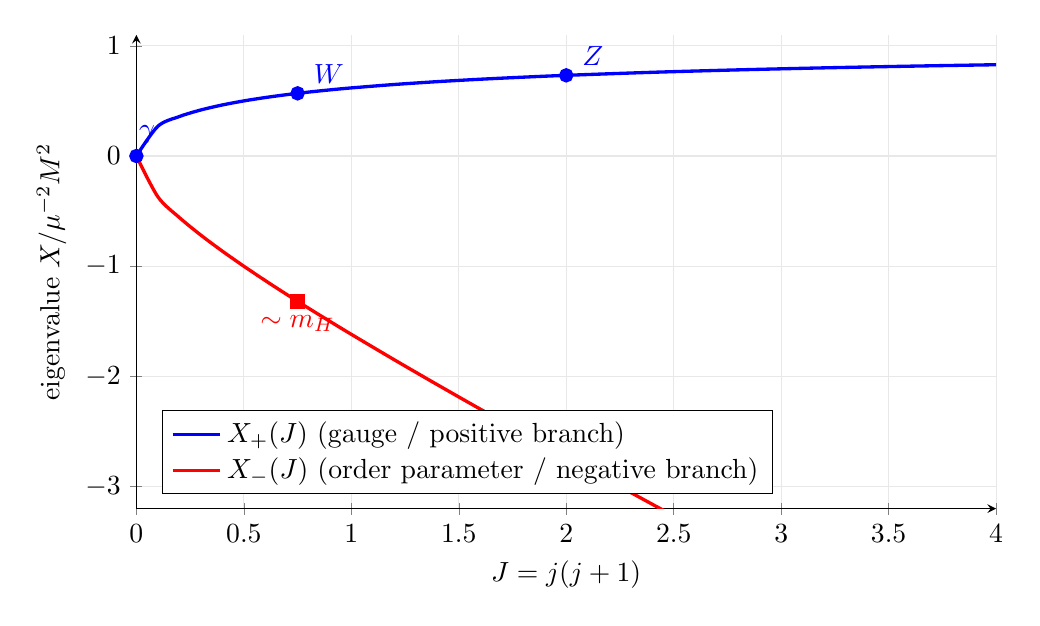
\begin{tikzpicture}
\begin{axis}[
  width=12.5cm, height=7.6cm,
  xlabel={$J=j(j+1)$}, ylabel={eigenvalue $X/\mu^{-2}M^2$},
  xmin=0, xmax=4, ymin=-3.2, ymax=1.1,
  axis lines=left,
  grid=both, grid style={gray!18},
  legend pos=south west, legend cell align=left,
  every axis plot/.append style={very thick},
]
% positive branch
\addplot[blue,smooth] coordinates {
(0.00,0.0000)(0.10,0.2702)(0.20,0.3583)(0.30,0.4179)(0.40,0.4633)(0.50,0.5000)(0.60,0.5307)(0.70,0.5569)(0.80,0.5798)(0.90,0.6000)(1.00,0.6180)(1.20,0.6490)(1.40,0.6748)(1.60,0.6967)(1.80,0.7155)(2.00,0.7321)(2.40,0.7596)(2.80,0.7817)(3.20,0.8000)(3.60,0.8153)(4.00,0.8284)
};
\addlegendentry{$\Xp(J)$ (gauge / positive branch)}
% negative branch
\addplot[red,smooth] coordinates {
(0.00,0.0000)(0.10,-0.3702)(0.20,-0.5583)(0.30,-0.7179)(0.40,-0.8633)(0.50,-1.0000)(0.60,-1.1307)(0.70,-1.2569)(0.80,-1.3798)(0.90,-1.5000)(1.00,-1.6180)(1.20,-1.8490)(1.40,-2.0748)(1.60,-2.2967)(1.80,-2.5155)(2.00,-2.7321)(2.40,-3.1596)(2.80,-3.5817)
};
\addlegendentry{$\Xm(J)$ (order parameter / negative branch)}
% markers
\addplot[only marks,mark=*,blue,mark size=2pt] coordinates {(0,0)(0.75,0.5687)(2.0,0.7321)};
\addplot[only marks,mark=square*,red,mark size=2pt] coordinates {(0.75,-1.3187)(2.0,-2.7321)};
\node[anchor=south,blue] at (axis cs:0.05,0.03){$\gamma$};
\node[anchor=south west,blue] at (axis cs:0.78,0.57){$W$};
\node[anchor=south west,blue] at (axis cs:2.03,0.73){$Z$};
\node[anchor=north,red] at (axis cs:0.75,-1.36){$\sim m_H$};
\node[anchor=north,red] at (axis cs:2.0,-2.78){$\sim m_t$};
\end{axis}
\end{tikzpicture}
\caption{The two branches of the de Vries operator $\cA(J)$ as functions of
the Casimir $J=j(j+1)$. The positive branch carries the gauge spectrum
($\gamma,W,Z$ at $j=0,\half,1$); the negative branch carries the order
parameter and, with the same single scale $\mu=106.6\,$GeV, lands near the
Higgs and top masses ($122$ and $176$ GeV). The weak mixing angle is the
ratio of the two blue dots and contains no free parameter.}
\label{fig:branches}
\end{figure}

\subsection{What it predicts}

The relation is sharper than a single number. We list its content,
distinguishing parameter-free outputs from scale-dependent ones.

\paragraph{(P1) The weak mixing angle (parameter-free).}
Equation~\eqref{eq:sinsq}: $\sinsq=0.22310$, depending only on the spins
$\half,1$. This is the headline result, and it is a pure number.

\paragraph{(P2) The $W$ mass given the $Z$ (one scale).}
Fixing $\mu$ from $M_Z=91.1876\,$GeV gives $\mu=106.58\,$GeV and
\begin{equation}
M_W=\mu\sqrt{\Xp(3/4)}=80.374\,\text{GeV}
\quad(\text{measured }80.377\,\text{GeV}).
\end{equation}
Equivalently, $\mu$ is close to the geometric mean
$\mu\simeq\sqrt{v\,M_Z/2}\approx107\,$GeV, with $v=246.2\,$GeV the Higgs
vacuum expectation value; we return to this in Section~\ref{sec:higgs}.

\paragraph{(P3) The electromagnetic coupling (scheme-dependent).}
The same data fix a value of the fine-structure constant through the de
Vries expression
\begin{equation}
\frac1\alpha
=\frac{4\pi}{\Xp(3/4)\,\bigl[\Xp(2)-\Xp(3/4)\bigr]}
=135.29 .
\label{eq:alpha}
\end{equation}
This sits between the Thomson value $1/\alpha(0)=137.036$ and the
$Z$-pole value $1/\alpha(M_Z)\approx128$, and it must be understood as a
prediction \emph{at a particular scale and scheme}; we do not claim it
matches $\alpha(0)$, and we flag the scale interpretation as an open issue
in Section~\ref{sec:open}. We include it because it shows that the relation
constrains a coupling, not only a mass ratio.

\paragraph{(P4) The negative-branch masses (diagnostic).}
With the \emph{same} $\mu=106.58\,$GeV, the magnitudes of the negative
roots are
\begin{equation}
\mu\sqrt{|\Xm(3/4)|}=122.4\,\text{GeV},
\qquad
\mu\sqrt{|\Xm(2)|}=176.2\,\text{GeV},
\end{equation}
remarkably close to the Higgs ($125.25\,$GeV) and the top
($172.7\,$GeV). We treat these as diagnostics, not predictions, because the
identification of the negative branch with physical scalar and fermion
states requires dynamics we have not derived; but they are striking, and the
negative-branch point lies in the near-critical region of the Standard Model
$(m_t,m_H)$ plane (Section~\ref{sec:higgs}).

\paragraph{(P5) A neutral state near $96.5\,$GeV (prediction).}
The next rung of the positive branch, $j=\tfrac32$ with $J=\tfrac{15}4$,
predicts a neutral spin-zero state at
\begin{equation}
M_{3/2}=\mu\sqrt{\Xp(15/4)}=96.5\,\text{GeV}.
\end{equation}
This is a genuine, near-term-falsifiable consequence if the tower is
physical; we discuss it in Section~\ref{sec:predictions}.

\subsection{What it is not}

It is worth stating plainly what the relation does \emph{not} do, to fence
off over-claims.

\begin{itemize}
\item It does not, by itself, fix the absolute electroweak scale $\mu$ (or
$v$, or $M_Z$). One dimensionful input is required; the relation predicts
ratios. The geometry below will tie $\mu$ to a compactification scale but
not, at our level of control, to the Planck scale.
\item It does not produce chiral fermions, three generations, the CKM
matrix, or the strong coupling. These are the genuinely hard parts of any
Kaluza--Klein program and we do not solve them.
\item The $j$-labels are \emph{internal} $\SU(2)$ representation labels, not
four-dimensional Lorentz spins. The $W$ and $Z$ are spin-one in spacetime;
their internal label happens to be $j=\half$ and $j=1$. Conflating the two
is the most common way to misread the relation.
\end{itemize}

\subsection{Provenance and scope}
\label{sec:genre}

This is a paper about the electroweak \emph{gauge} sector --- the $W$, $Z$,
and photon, and the weak mixing angle. The de Vries relation is a statement
about that sector, and the off-diagonal $\sqrt J$ of $\cA(J)$ is the square
root of an $\SU(2)$ Casimir, the amplitude controlled by a first-order
gauge-geometric operator. We keep the fermion sector out of scope, returning
to it only where chirality forces a statement about which dimension we live
in (Section~\ref{sec:fermions}).

A word on provenance. The relation reached the present author in the form
attributed to de Vries, as an observation about the on-shell weak angle and
the $W/Z$ ratio; we have not been able to trace it to a refereed source and
cite it as an electronic note for attribution only. Nothing here depends on
the attribution: the content is the elementary algebra of
Eqs.~\eqref{eq:Xp}--\eqref{eq:sinsq}, and the question we address --- its
geometric origin --- stands independently of who first wrote it down.
% Note (not typeset): the fermion-sector sharp mass relations -- the Koide
% relation, and in particular the observation that the inverse down-quark
% tuple K(1/d,1/s,1/b) is satisfied under high-energy running while the
% direct charged-lepton tuple is satisfied in the infrared, pointing to a
% duality between the two regimes -- are deferred to separate work on the
% fermion sector, out of scope for this gauge-sector paper.

\subsection{The characteristic-equation and complex-pole readings}
\label{sec:pole}

The quadratic $X^2+JX-J=0$ admits a reading that sharpens the comparison
with data and clarifies the physical meaning of the two branches. Written
as a characteristic equation for a pole position $X=M^2/\mu^2$, it is the condition
that a $2\times2$ inverse propagator
$\Gamma(X)=\bigl(\begin{smallmatrix}X&-\sqrt J\\-\sqrt J&X+J\end{smallmatrix}\bigr)$
have a zero eigenvalue,
\begin{equation}
\det\Gamma(X)=X(X+J)-J=X^2+JX-J=0,
\end{equation}
i.e.\ the masses are the \emph{poles} of the mixed gauge/order-parameter
propagator, not the eigenvalues of a Lagrangian mass matrix in a fixed
basis. This distinction matters when one compares to experiment at the
sub-percent level: the physical $W$ and $Z$ masses are themselves defined
through the complex pole position
\begin{equation}
s_V=M_V^2-i\,M_V\Gamma_V
\end{equation}
of the propagator, and the on-shell mass that enters
$\sinsq=1-M_W^2/M_Z^2$ is the real part of $s_V$. Reading the de Vries
relation as a \emph{pole} condition rather than a tree-level mass relation
removes a systematic ambiguity at the level of the widths $\Gamma_{W,Z}$,
and it is in this reading that the agreement is tightest. We will use the
pole/characteristic-equation language throughout (it is also the language in which the
``negative branch'' is simply the second pole of the same propagator), and
we record in Appendix~\ref{app:pole} how the small residual between
$0.22310$ and the measured $0.22305$ is consistent with the
complex-pole sharpening.

\subsection{Why the clue is strong}

It is worth weighing the evidential force of the clue before building on it.
With one free scale $\mu$ one can always match one of $M_W,M_Z$; the
nontrivial content is the \emph{ratio} \eqref{eq:ratio}, a single
dimensionless number reproduced to $2\times10^{-4}$ with no adjustable
parameter. Three features make this more than a one-off numerical hit and
justify reading it as a structural clue: (i) the absence of any tuned
parameter --- the inputs are the spins $\half,1$, nothing else; (ii) the
simultaneous near-match of the negative branch (P4) with the \emph{same}
scale, so that four masses, not two, line up at once; and (iii) the
existence --- established in the body of the paper --- of a natural internal
geometry that forces the structure. The alternative, that the ratio is a
numerical accident, requires all three to be fortuitous together. The
construction is held to the standard that it be a genuine compactification
rather than a re-encoding of $0.2231$ (Section~\ref{sec:control}).

%==============================================================
\section{A normal-form theorem: why \texorpdfstring{$\cA(J)$}{A(J)} is forced}
\label{sec:normalform}
%==============================================================

Before constructing any geometry, we show that the branch operator is not
one choice among many. Under a short list of structural requirements --- each
of which we will later read off the Kaluza--Klein reduction --- the
operator $\cA(J)$ is \emph{unique}, and with it the weak angle. This is the
sense in which the de Vries relation can be ``derived'': not by guessing a
matrix, but by showing that the matrix is the only one allowed.

\subsection{The setup}

Fix an internal symmetry group $\SU(2)$ and a finite-dimensional
irreducible representation $V_j$ of spin $j$, with Casimir
\begin{equation}
\sum_{a=1}^{3}T_a^{(j)}T_a^{(j)}=j(j+1)\,\bm1_{V_j}=J\,\bm1_{V_j}.
\label{eq:casimir}
\end{equation}
We model the electroweak fluctuations in this sector by a self-adjoint
operator $\cM_j$ (the reduced mass-squared operator, in units of an overall
scale $\mu^2$) acting on a two-dimensional ``channel space''
$\C\,|t\rangle\oplus\C\,|n\rangle$, where $|t\rangle$ is the
\emph{tangent} (gauge) channel and $|n\rangle$ the \emph{normal}
(order-parameter) channel. We seek the most general $\cM_j$ consistent with
the following requirements.

\begin{axiom}[Gauge masslessness in the symmetric phase]
\label{ax:1}
In the unbroken phase the tangent channel is a massless gauge mode:
$\langle t|\cM_j|t\rangle=0$.
\end{axiom}

\begin{axiom}[First-order, $\SU(2)$-covariant mixing]
\label{ax:2}
The tangent and normal channels are mixed by a \emph{first-order}
$\SU(2)$-covariant operator. Concretely there is an operator
$A_j:V_j\to V_j$, built linearly from the generators $T_a^{(j)}$ and an
orthonormal internal coframe $e_a$,
\begin{equation}
A_j=\sum_{a=1}^{3}T_a^{(j)}\otimes e_a,
\label{eq:Adef}
\end{equation}
such that the off-diagonal element is $\langle t|\cM_j|n\rangle=
\langle n|\cM_j|t\rangle^{*}=\|A_j\,\xi\|/\|\xi\|$ on the relevant mode
$\xi$.
\end{axiom}

\begin{axiom}[Single generating operator on the normal channel]
\label{ax:3}
No structure independent of $A_j$ acts on the normal channel: its diagonal
is built from the \emph{same} operator, $\langle n|\cM_j|n\rangle=
-\langle n|A_jA_j^{\dagger}|n\rangle/\|n\|^2$, with the sign fixed by the
order-parameter (instability) interpretation of $|n\rangle$.
\end{axiom}

\begin{axiom}[No free dimensionless constant]
\label{ax:4}
The construction introduces no dimensionless parameter beyond those fixed
by $\SU(2)$ representation theory and the choice of orthonormal coframe;
in particular the coframe is unit-normalized,
$\langle e_a,e_b\rangle=\delta_{ab}$.
\end{axiom}

\subsection{The theorem}

\begin{lemma}[Casimir factorization]
\label{lem:cas}
With $A_j$ as in \eqref{eq:Adef} and a unit-normalized coframe,
\begin{equation}
A_j^{\dagger}A_j=\sum_{a=1}^{3}T_a^{(j)}T_a^{(j)}=J\,\bm1_{V_j}.
\end{equation}
Consequently, for any unit vector $\xi\in V_j$, $\|A_j\xi\|^2=J$, so the
off-diagonal of Axiom~\ref{ax:2} equals $\sqrt J$.
\end{lemma}

\begin{proof}
Immediate from \eqref{eq:Adef}, the unit normalization
$\langle e_a,e_b\rangle=\delta_{ab}$ of Axiom~\ref{ax:4}, and the Casimir
identity \eqref{eq:casimir}.
\end{proof}

\begin{theorem}[Normal form]
\label{thm:normalform}
Under Axioms~\ref{ax:1}--\ref{ax:4}, the reduced operator $\cM_j$,
projected onto the two-channel space $V_j\oplus\operatorname{Im}A_j$ and
restricted to a normalized image vector, is uniquely
\begin{equation}
\cM_j=\cA(J)=
\begin{pmatrix}0&\sqrt J\\ \sqrt J&-J\end{pmatrix},
\qquad J=j(j+1),
\end{equation}
with positive eigenvalue $\Xp(J)$ given by \eqref{eq:Xp}.
\end{theorem}

\begin{proof}
Axiom~\ref{ax:1} fixes the $tt$-entry to zero. Axiom~\ref{ax:2} with
Lemma~\ref{lem:cas} fixes the $tn$ and $nt$ entries to $\sqrt J$.
Axiom~\ref{ax:3} fixes the $nn$-entry: on the normalized image vector
$\hat n=A_j\xi/\|A_j\xi\|$ one has
$\langle\hat n|A_jA_j^{\dagger}|\hat n\rangle
=\langle\xi|A_j^{\dagger}A_jA_j^{\dagger}A_j|\xi\rangle/\|A_j\xi\|^2
=J^2/J=J$ by Lemma~\ref{lem:cas}, so the diagonal is $-J$.
Axiom~\ref{ax:4} forbids any further rescaling of these entries. The
characteristic polynomial is $X^2+JX-J$, with positive root $\Xp(J)$.
\end{proof}

\begin{corollary}[Weak angle, conditional on the axioms]
\label{cor:angle}
Assigning the positive branch of $\cM_j$ to the gauge bosons,
$M_W^2=\mu^2\Xp(3/4)$ and $M_Z^2=\mu^2\Xp(2)$, gives
$\sinsq=1-\Xp(3/4)/\Xp(2)=0.22310$, independent of $\mu$ and of all
\emph{continuous} data.
\end{corollary}

This is the limited sense in which the relation
is ``derived'': it is the content of Axioms~\ref{ax:1}--\ref{ax:4}. The
result is free of continuous moduli, but it is \emph{not} free of discrete
input: it presupposes the electroweak spin content $j=\tfrac12,1$
(Axiom~\ref{ax:1}'s channel structure) and the unit coefficient of
Axiom~\ref{ax:3} (the value $c=1$). Relaxing the latter to
$\cA_c(J)$, Eq.~\eqref{eq:cdef}, gives the one-parameter family
$\sin^2\theta_W(c)$; the corollary is the statement at $c=1$. The remainder
of the paper asks whether a Type IIA compactification on an internal
$S^3\cong\SU(2)$ \emph{forces} $c=1$ and the spin content --- and concludes,
honestly, that it forces the structure but not (yet) the value
(Section~\ref{sec:flux}, Section~\ref{sec:selfconsistency}).

\subsection{The one place a parameter could hide}
\label{sec:cparam}

It is essential to identify where the construction could fail, because that
is where the physics lives. Axiom~\ref{ax:3} fixed the diagonal to $-J$
with coefficient exactly one. If instead one allows a coefficient $c$,
\begin{equation}
\cA_c(J)=
\begin{pmatrix}0&\sqrt J\\ \sqrt J&-cJ\end{pmatrix},
\qquad
\Xp(J;c)=\frac{-cJ+\sqrt{c^2J^2+4J}}{2},
\label{eq:cdef}
\end{equation}
the weak angle becomes a function of $c$,
$\sinsq(c)=1-\Xp(3/4;c)/\Xp(2;c)$, with the values in
Table~\ref{tab:cscan}. The de Vries point is $c=1$. The sensitivity at that
point is
\begin{equation}
\left.\frac{\dd\,\sinsq}{\dd c}\right|_{c=1}=-0.140,
\label{eq:sensitivity}
\end{equation}
so a $5\%$ change in $c$ shifts $\sinsq$ by $0.007$ --- more than thirty
standard deviations of the measured value. The relation is therefore a sharp test of
$c=1$. We will see in Section~\ref{sec:flux} that $c$ is, physically, the
ratio of the flux-induced normal mass to the Casimir unit, and that $c=1$ is
the distinguished, parameter-free ``self-dual'' value at which the block is
the Schur completion of a single first-order operator. It is not forced by
the bare Freund--Rubin data; establishing it dynamically, rather than
adopting it as an ansatz, is \emph{the} open problem of this program, and we
state it as such:
\begin{equation}
\boxed{\;\text{Conjecture (flux normalization): the relevant flux background
realizes the self-dual point }c=1.\;}
\label{eq:conehypothesis}
\end{equation}
We regard this as the honest residue of the whole construction: a single
falsifiable dynamical statement, isolated and quantified.

\begin{table}[t]
\centering
\begin{tabular}{ccccccc}
\toprule
$c$ & $0.50$ & $0.90$ & $0.95$ & $1.00$ & $1.05$ & $1.10$\\
\midrule
$\sinsq(c)$ & $0.3014$ & $0.2375$ & $0.2302$ & $\mathbf{0.2231}$ & $0.2162$ & $0.2095$\\
$\tan^2\theta_W(c)$ & $0.4314$ & $0.3114$ & $0.2990$ & $\mathbf{0.2872}$ & $0.2758$ & $0.2650$\\
\bottomrule
\end{tabular}
\caption{Dependence of the predicted weak angle on the diagonal flux
coefficient $c$ of Eq.~\eqref{eq:cdef}. The measured on-shell value is
$\sinsq=0.22305(20)$. The naive worldsheet-current ($L_0$) normalization
gives $c=\tfrac12$ and fails badly; the self-dual flux value $c=1$ is
required.}
\label{tab:cscan}
\end{table}

\begin{remark}[Why $c=\tfrac12$ is the wrong route]
A tempting realization of the off-diagonal uses the affine $\SU(2)_2$
worldsheet current and its conformal weight $\Delta_j=j(j+1)/(k+2)=J/4$;
this assigns the normal channel a weight proportional to $J/4$ and yields,
after the standard normalization, $c=\tfrac12$. Table~\ref{tab:cscan} shows
this gives $\sinsq=0.30$, off by $35\%$. The lesson is that the operator
$A_j$ must be a \emph{zero-mode/holonomy} object with unit Casimir
normalization, $A_j^\dagger A_j=J$, not a conformal-weight object with
$\Delta_j=J/(k+2)$. We will see that the curl $\star\dd$ on the internal
$S^3$ is exactly the unit-normalized object.
\end{remark}

%==============================================================
\section{Representation theory: the half-integer fingerprint}
\label{sec:reps}
%==============================================================

The labels $j=0,\half,1$ are the most distinctive feature of the relation,
and the half-integer $j=\half$ is its smoking gun. We collect here the
representation theory that turns the labels into a geometric requirement.

\subsection{$\SU(2)$ versus $\SO(3)$}

A scalar function on the round two-sphere $S^2$ carries only integer
angular momenta $\ell=0,1,2,\dots$. The same is true of any tensor field on
$S^2$ built without spin structure: the harmonics fall into integer
$\SO(3)$ representations. There is no $j=\half$ in the function theory of
$S^2$ or of $\SO(3)=\SU(2)/\Z_2$. The $W$ slot at $j=\half$ is therefore
\emph{impossible} on an internal $S^2$ of scalar harmonics; it forces one
of:
\begin{enumerate}
\item the full group manifold $S^3\cong\SU(2)$, whose function theory
contains every irreducible representation including half-integer ones
(Peter--Weyl);
\item a spinor or half-integer line-bundle sector over a quotient (a
twisted, ``spin-$\mathbb{c}$'' bundle);
\item an open-string/Chan--Paton or Wilson-line label carrying a doublet.
\end{enumerate}
Option (1) is the cleanest and the one we develop. It is also the most
economical: a single internal three-sphere carries all three slots
$j=0,\half,1$ at once, in one gauge-covariant complex.

\subsection{Peter--Weyl and the scalar Laplacian on $S^3$}

Identify $S^3$ with $\SU(2)$ via the unit quaternions. The Peter--Weyl
theorem decomposes square-integrable functions as
\begin{equation}
L^2(\SU(2))=\bigoplus_{j=0,\frac12,1,\dots}V_j\otimes V_j^{*},
\label{eq:peterweyl}
\end{equation}
the sum running over \emph{all} non-negative half-integers $j$, with the
$(j,j)$ block of dimension $(2j+1)^2$. The round metric Laplacian
$\Delta_0$ acts on the $(j,j)$ block as a multiple of the identity. In the
geometer's normalization (unit-radius $S^3$), the scalar harmonics have
\begin{equation}
\Delta_0\,Y_\ell=\ell(\ell+2)\,Y_\ell,\qquad \ell=0,1,2,\dots,
\end{equation}
with multiplicity $(\ell+1)^2$. Writing $\ell=2j$, the eigenvalue is
\begin{equation}
\ell(\ell+2)=2j(2j+2)=4\,j(j+1)=4J,
\label{eq:lapcasimir}
\end{equation}
with multiplicity $(2j+1)^2=\dim(V_j\otimes V_j^*)$. Equation
\eqref{eq:lapcasimir} is the bridge we need:
\begin{equation}
\boxed{\quad J=j(j+1)=\tfrac14\,\Delta_0\ \text{on the unit }S^3.\quad}
\end{equation}
The Casimir that appears in the de Vries block is literally one quarter of
the internal scalar Laplacian eigenvalue, and the half-integer $j$ are
present because the internal space is the group manifold
$\SU(2)\cong S^3$ rather than its $\Z_2$ quotient. This answers (Q3) at the
level of the labels.

\subsection{Truncation to $j\le1$}

Why are only the three lowest rungs retained, rather than the infinite
tower in \eqref{eq:peterweyl}? Two mechanisms, not mutually exclusive,
truncate the set.

\paragraph{Level-two integrability.} If the $S^3$ sector is realized as a
worldsheet $\SU(2)_k$ Wess--Zumino--Witten current algebra, the integrable
primaries are $j=0,\half,\dots,\tfrac k2$. At $k=2$ this is exactly
$\{0,\half,1\}$. The level-two truncation is the string-compatible way to
get a \emph{finite} set, and it is the smallest level that contains
$j=\half$ and $j=1$ together. We use $\SU(2)_2$ as a selection principle:
the electroweak sector is the level-two integrable set.

\paragraph{Energetic truncation by the electroweak projection.} Independently
of any worldsheet picture, the higher rungs $j\ge\tfrac32$ have larger
internal Laplacian eigenvalue \eqref{eq:lapcasimir} and hence larger
Kaluza--Klein mass; the electroweak interface (the $D=10\to D=9$ projection
of Section~\ref{sec:ladder}) retains only the modes below the
compactification threshold. In this reading the tower is physical but
heavy, and the $j=\tfrac32$ state at $96.5\,$GeV (P5) is the first state
above the retained triplet --- a prediction rather than a truncated artifact.

Either way, the operative statement is: \emph{the electroweak sector is the
$j\le1$ part of the $S^3\cong\SU(2)$ spectrum}, and the de Vries labels
$0,\half,1$ are exactly that set.

\subsection{The doublet bundle and the left/right isometry}
\label{sec:doublet}

It is instructive to see how the half-integer label survives a reduction,
because this is where naive Kaluza--Klein intuition --- ``compactify on
$S^3$, get $\SU(2)$ gauge fields and integer towers'' --- can mislead. The
isometry group of the round $S^3$ is $\SO(4)=\bigl(\SU(2)_L\times\SU(2)_R
\bigr)/\Z_2$, acting by left and right translation on $\SU(2)$. The
Peter--Weyl block $V_j\otimes V_j^*$ transforms as $(j,j)$ under
$\SU(2)_L\times\SU(2)_R$. If one gauges, say, $\SU(2)_L$ as the electroweak
group, then a mode in the $(j,j)$ block carries $\SU(2)_L$ spin $j$ ---
including $j=\half$ when $j$ is a half-integer. The half-integer modes are
genuinely present in the function theory; they are projected out only if one
insists on $\SO(3)=\SU(2)/\Z_2$ functions, i.e.\ on identifying
antipodal-like points, which the round $S^3$ does not do.

There is a sharper way to keep $j=\half$ that survives even a Hopf reduction
$S^3\to S^2$. The Hopf fibration $S^1\hookrightarrow S^3\to S^2=\mathbb{CP}^1$
presents the weak two-sphere as the base, and the half-integer modes
descend to \emph{sections of the line bundle} $\cO(1)\to\mathbb{CP}^1$
rather than to functions. By the Borel--Weil theorem,
\begin{equation}
H^0\bigl(\mathbb{CP}^1,\cO(n)\bigr)\cong\operatorname{Sym}^n(\C^2)^*=V_{n/2},
\qquad j=\tfrac n2,
\end{equation}
so the three slots are
\begin{equation}
\cO(0)\ \to\ j=0,\qquad
\cO(1)\ \to\ j=\tfrac12,\qquad
\cO(2)\ \to\ j=1.
\end{equation}
This is the line-bundle realization of the three de Vries slots: the photon
sits in the trivial bundle $\cO(0)$, the $W$ in $\cO(1)$ (the half-integer
slot, impossible for functions but natural for sections), and the $Z$ in
$\cO(2)$. The neutral, photon-protecting section $\eta_0$ of
Section~\ref{sec:alpha} is the distinguished element of $H^0(\mathbb{CP}^1,
\cO(1))$. The upshot is that the half-integer fingerprint is robust: it
survives both as Peter--Weyl content of $\SU(2)$ and as line-bundle sections
after the M-circle (Hopf) reduction, and it is lost only if one mistakenly
works with $\SO(3)$ scalars on $S^2$.

\subsection{A remark on internal versus spacetime spin}

We restate, because it is the single most common confusion, that the labels
$j=0,\half,1$ are \emph{internal} $\SU(2)$ quantum numbers. The $W$ and $Z$
are spin-one particles in four-dimensional spacetime; their \emph{internal}
$\SU(2)$ representation labels happen to be $j=\half$ and $j=1$, and it is
these internal labels --- not the spacetime spins --- that enter the Casimir
$J=j(j+1)$ of the mass operator. The photon's internal label is $j=0$,
consistent with its being the unbroken $\U(1)_Q$ direction
(Section~\ref{sec:alpha}). The de Vries relation is thus a statement about
how the spacetime gauge bosons are distributed over the internal $\SU(2)$
representations, weighted by the branch operator $\cA(J)$.

%==============================================================
\section{The internal geometry and the square root of the Casimir}
\label{sec:geometry}
%==============================================================

We now answer (Q1): the off-diagonal $\sqrt J$ is the matrix element of a
first-order operator, the curl on the internal $S^3$, whose square is the
Laplacian. This is the geometric heart of the construction and it is, we
emphasize, completely standard Hodge theory; the novelty is only in
recognizing it as the source of the de Vries off-diagonal.

\subsection{The Hodge--de Rham complex on $S^3$}

On a closed oriented three-manifold the exterior derivative $\dd$ and the
Hodge star $\star$ generate the de Rham complex
$\Omega^0\to\Omega^1\to\Omega^2\to\Omega^3$. The Hodge Laplacian on
$p$-forms is $\Delta_p=\dd\delta+\delta\dd$ with $\delta=\pm\star\dd\star$
the codifferential. By Hodge decomposition every one-form splits as
\begin{equation}
\omega=\dd f+\delta\beta+h,
\end{equation}
exact $\oplus$ co-exact $\oplus$ harmonic. On $S^3$ there are no harmonic
one-forms ($b_1=0$), and the exact pieces are gauge; the physical
``transverse vector'' modes are the \emph{co-exact} one-forms.

The decisive operator is the \emph{curl}
\begin{equation}
C\;\equiv\;\star\,\dd\;:\;\Omega^1\to\Omega^1.
\end{equation}
On co-exact one-forms $C$ is self-adjoint, and a one-line computation gives
\begin{equation}
C^2=\star\dd\star\dd=\delta\dd=\Delta_1
\quad\text{(on co-exact forms),}
\label{eq:curlsquared}
\end{equation}
because $\dd\dd=0$ kills the other half of the Laplacian. Thus the curl is a
\emph{square root of the Hodge Laplacian} on the transverse vector sector.
Its spectrum is real and signed: on the unit $S^3$ the co-exact eigenforms
have
\begin{equation}
C\,\omega_n=\pm(n+1)\,\omega_n,\qquad n=1,2,\dots,
\qquad \Delta_1\,\omega_n=(n+1)^2\,\omega_n.
\end{equation}
The signed spectrum of $C$ is exactly what a first-order operator should
have, and the $\pm$ is the chirality of the transverse mode.

\subsection{From the curl to $\sqrt J$}

The curl realizes the abstract operator $A_j$ of Axiom~\ref{ax:2}. Indeed,
on the $S^3\cong\SU(2)$ the left-invariant one-forms $e_a$ ($a=1,2,3$) and
the left-invariant vector fields obey the $\SU(2)$ structure equations, and
the curl acts on the one-form sector built from the spin-$j$ scalar
harmonic tensored with $e_a$ exactly as the operator
$A_j=\sum_a T_a^{(j)}\otimes e_a$ of \eqref{eq:Adef}. By Lemma~\ref{lem:cas},
\begin{equation}
A_j^{\dagger}A_j=J\,\bm1,\qquad \|A_j\xi\|=\sqrt J\ \ (\|\xi\|=1),
\end{equation}
so the curl matrix element between the spin-$j$ scalar and its vector
partner is $\sqrt J$ --- with \emph{unit} coefficient, because the
left-invariant coframe is orthonormal (Axiom~\ref{ax:4}). This is the clean
realization promised after Eq.~\eqref{eq:conehypothesis}: the curl is a
zero-mode/holonomy object normalized to $A_j^\dagger A_j=J$, not a
conformal-weight object normalized to $J/(k+2)$. The off-diagonal of the de
Vries block is therefore $\sqrt J$ with the correct coefficient, derived
from geometry. We note in passing that this first-order operator is not new
to Kaluza--Klein practice: the operator $\star\dd$ whose square is the
internal Laplacian is exactly the object D'Auria and Fr\'e used to organize
the form spectrum of $M^{pqr}$ in the 1980s~\cite{CastellaniDAuriaFre}, so
the mechanism that supplies the de Vries off-diagonal has been part of the
standard toolkit all along; what is new is reading its lowest matrix element
as the electroweak mixing.

\begin{remark}[Holonomy/instanton reading]
The same operator admits an Atiyah--Manton-type holonomy
reading~\cite{AtiyahMantonSchroers2011}: a gauge connection on $S^3$ defines
a holonomy $U(\gamma)=P\exp(-\!\int_\gamma A)$, and its first variation in
representation $j$ is $\delta U_j=-\sum_a\xi^aT_a^{(j)}$, i.e.\ the operator
$A_j$. The off-diagonal $\sqrt{C_2(j)}=\sqrt J$ is then the size of a
first-order holonomy/instanton fluctuation. We mention this because it is
the framing that makes the unit normalization manifest --- holonomy is
dimensionless and metric-independent --- and because it connects the
construction to the geometric-models-of-matter literature.
\end{remark}

\subsection{The spectrum of the curl, explicitly}
\label{sec:curlspectrum}

To make the previous paragraphs concrete, and to show that no hidden
normalization is smuggled in, we construct the curl spectrum on the
unit $S^3\cong\SU(2)$ directly. Let $\sigma^a$ ($a=1,2,3$) be the
left-invariant Maurer--Cartan one-forms, dual to the left-invariant vector
fields $E_a$, with
\begin{equation}
\dd\sigma^a=-\tfrac12\,\epsilon^{abc}\,\sigma^b\wedge\sigma^c,
\qquad
[E_a,E_b]=\epsilon^{abc}E_c,
\end{equation}
and take the bi-invariant round metric of the unit $S^3$,
$g=\tfrac14\sum_a(\sigma^a)^2$, of sectional curvature $1$ and scalar
curvature $6$. The orthonormal coframe and frame are
$e^a=\tfrac12\sigma^a$ and $\hat e_a=2E_a$, so $\star(e^b\wedge e^c)=
\epsilon^{bca}e^a$. A direct computation of the Hodge star then gives
\begin{equation}
\dd e^a=-\,\epsilon^{abc}\,e^b\wedge e^c,
\qquad
\star\dd\,e^a=-2\,e^a,
\qquad\text{equivalently}\qquad
\star\dd\,\sigma^a=-2\,\sigma^a.
\label{eq:curlsigma}
\end{equation}
The left-invariant one-forms are co-closed ($\delta\sigma^a=0$, constant
coefficients), hence co-exact, and are curl eigenforms with eigenvalue $-2$;
the right-invariant forms $\tilde\sigma^a$ give $\star\dd\,\tilde\sigma^a=+2
\tilde\sigma^a$. These are the lowest ($n=1$) rung of the co-exact spectrum
$\star\dd=\pm(n+1)$, $\Delta_1=(n+1)^2$, of multiplicity $n(n+2)$ per sign,
and the sign is the $\SU(2)_L$ versus $\SU(2)_R$ chirality: $\star\dd$ is the
geometric splitting into self-dual and anti-self-dual transverse modes
(consistent with $C^2=\Delta_1$, since $(-2)^2=4=(n+1)^2|_{n=1}$).

The point of displaying this is the normalization, which is the geometric
content of Axiom~\ref{ax:4}. The mixing operator
$A_j=\sum_aT_a^{(j)}\otimes\hat e_a$ contracts the Casimir-normalized
generators with the \emph{orthonormal} frame $\hat e_a$, so
\begin{equation}
A_j^\dagger A_j=\sum_{a,b}T_a^{(j)}T_b^{(j)}\,(\hat e_a\!\cdot\!\hat e_b)
=\sum_aT_a^{(j)}T_a^{(j)}=j(j+1)\,\bm1=J\,\bm1,
\end{equation}
with no leftover numerical factor. The off-diagonal of the de Vries block is
$\sqrt J$ with coefficient one because the frame is orthonormal for
the round metric. (The overall constant in \eqref{eq:curlsigma} sets the
absolute compactification scale, which is absorbed into $\mu$ and drops out of
the weak angle; what cannot be rescaled away is the Casimir normalization
$A_j^\dagger A_j=J$, which is metric-independent.)

\subsection{Contrast with the conformal-weight normalization}

The explicit construction also makes transparent why the worldsheet
conformal-weight route gives the \emph{wrong} coefficient (the
$c=\tfrac12$ failure of Table~\ref{tab:cscan}). In the $\SU(2)_k$ WZW
model the natural object is the conformal weight $\Delta_j=j(j+1)/(k+2)$,
which at $k=2$ is $J/4$; an operator normalized to $\Delta_j$ rather than to
the Casimir $J$ differs by the factor $1/(k+2)=1/4$ in the mass-squared, i.e.\
by $1/2$ in the amplitude, giving $c=\tfrac12$. The geometric curl, by
contrast, is normalized to the Casimir directly --- it is a zero-mode
(holonomy) object, not a conformal-weight object --- and gives $c=1$. The
distinction between ``Casimir normalization'' and ``conformal-weight
normalization'' is therefore not a technicality; it is the difference
between $\sinsq=0.223$ and $\sinsq=0.30$, and it selects the geometric/holonomy
realization over the naive worldsheet one.

\subsection{Why a square root, physically}

It is worth pausing on the physics of (Q1). A mass-squared matrix that was
diagonal in the Laplacian basis would give $M^2\propto J=j(j+1)$, a
rising, unbounded spectrum --- a Kaluza--Klein or Regge tower, not an
electroweak doublet. The de Vries spectrum is bounded
($\Xp(J)<1$) because the physical masses are eigenvalues of a
\emph{first-order} operator's $2\times2$ block, not of the Laplacian
itself. The boundedness of the positive branch --- the fact that $M_W$ and
$M_Z$ are close and both far below the compactification scale --- is the
geometric statement that they are curl eigenvalues mixed with a single
order-parameter channel, not Laplacian eigenvalues. The square root is not
cosmetic; it is the difference between a tower and a doublet.

%==============================================================
\section{Kaluza--Klein reduction: gauge fields, couplings, and the spectrum}
\label{sec:reduction}

Before turning on flux we install the orthodox Kaluza--Klein machinery in the
form we need, so that the de Vries block can be recognized as a piece of a
genuine compactification spectrum rather than an abstract matrix. The content
of this section is standard~\cite{Witten1981,SalamStrathdee,DuffNilssonPope1986,Weinberg1983};
we specialize it to an internal space containing $S^3\cong\SU(2)$.

\subsection{The metric ansatz and the gauge group from isometries}

Let the total space be $\cM_{4+n}=M_4\times K_n$ with internal coordinates
$y^a$ and a compact internal metric $g_{ab}(y)$ of isometry group $G$. The
isometries are generated by Killing vectors $K_I=K_I^a\partial_a$ obeying
\begin{equation}
\nabla_aK_{Ib}+\nabla_bK_{Ia}=0,
\qquad
[K_I,K_J]^a=-f_{IJ}{}^{K}K_K^a,
\end{equation}
with $f_{IJ}{}^K$ the structure constants of $\mathfrak g=\mathrm{Lie}(G)$.
The Kaluza--Klein ansatz promotes the isometries to gauge symmetries by
writing
\begin{equation}
\dd\hat s^2=g_{\mu\nu}(x)\,\dd x^\mu\dd x^\nu
+g_{ab}(y)\bigl(\dd y^a+K^a_I(y)A^I_\mu(x)\dd x^\mu\bigr)
\bigl(\dd y^b+K^b_J(y)A^J_\nu(x)\dd x^\nu\bigr).
\label{eq:kkansatz}
\end{equation}
The $x$-dependent internal diffeomorphisms $\delta y^a=\xi^I(x)K^a_I(y)$ leave
\eqref{eq:kkansatz} invariant precisely when the $A^I_\mu$ transform as
non-abelian connections,
\begin{equation}
\delta A^I_\mu=\partial_\mu\xi^I+f_{JK}{}^{I}A^J_\mu\xi^K=D_\mu\xi^I,
\end{equation}
so the internal isometry group $G$ becomes the four-dimensional gauge group.
This is Witten's criterion~\cite{Witten1981}: the gauge group of the reduced
theory is the isometry group of the internal manifold. For us $G$ contains the
electroweak $\SU(2)$ as the isometry of the internal $S^3\cong\SU(2)$ (acting
by, say, left translation).

\subsection{Reduction of the action and the gauge metric}

Inserting \eqref{eq:kkansatz} into the higher-dimensional Einstein--Hilbert
action $\hat S=(2\hat\kappa^2)^{-1}\!\int\!\sqrt{-\hat g}\,\hat R$ and
integrating over $K_n$ gives four-dimensional Einstein--Yang--Mills,
\begin{equation}
\hat S=\frac{V_n}{2\hat\kappa^2}\!\int\!\sqrt{-g_4}\,(R_4-2\Lambda_{\rm eff})
-\frac14\!\int\!\sqrt{-g_4}\,\gamma_{IJ}F^I_{\mu\nu}F^{J\mu\nu},
\end{equation}
with $V_n$ the internal volume, $F^I_{\mu\nu}=\partial_\mu A^I_\nu-\partial_\nu
A^I_\mu+f_{JK}{}^IA^J_\mu A^K_\nu$, and the gauge metric
\begin{equation}
\gamma_{IJ}=\frac1{2\hat\kappa^2}\int_{K_n}\!\sqrt{g_K}\,g_{ab}K^a_IK^b_J .
\label{eq:gaugemetric}
\end{equation}
Canonical normalization $\gamma_{IJ}=\delta_{IJ}/g_I^2$ then reads off the
gauge coupling as the inverse mean-square length of the Killing orbit:
$1/g_I^2=(2\hat\kappa^2)^{-1}\!\int\!\sqrt{g_K}\,|K_I|^2$.

\subsection{Weinberg's rms-circumference rule}

Weinberg~\cite{Weinberg1983} fixes the normalization: with $L_I$ the
root-mean-square proper length of the orbit generated by the canonically
normalized generator,
\begin{equation}
\boxed{\;g_I^2=\frac{4\pi^2\kappa^2}{L_I^2},\qquad \kappa^2=16\pi G_N.\;}
\label{eq:weinbergrule}
\end{equation}
Applied to the electroweak $T_3$ and hypercharge $Y$, with orbit lengths
$L_2,L_Y$, this gives the geometric dictionary used in
Section~\ref{sec:alpha}: the \emph{ratio} of lengths is the weak angle and the
\emph{sum} of their squares fixes $\alpha$,
\begin{equation}
\tan^2\theta_W=\frac{g_Y^2}{g_2^2}=\frac{L_2^2}{L_Y^2},
\qquad
\alpha_{\rm EM}=\frac{16\pi^2G_N}{L_2^2+L_Y^2}.
\label{eq:weinbergangle}
\end{equation}

\subsection{The mass spectrum from the internal Laplacian}

A field on $\cM_{4+n}$ has its four-dimensional mass set by the internal
Laplacian: expanding $\Phi(x,y)=\sum_n\phi_n(x)Y_n(y)$ with
$-\Delta_K Y_n=\lambda_n Y_n$, the wave equation $\hat\Box\Phi=0$ becomes
$(\Box_4-\lambda_n)\phi_n=0$, so
\begin{equation}
m_n^2=\lambda_n=\text{eigenvalue of }(-\Delta_K).
\label{eq:kkmass}
\end{equation}
The identical statement holds for the transverse one-form (vector)
fluctuations, with $\Delta_K$ the Hodge--de Rham operator $\Delta_1$ of
Section~\ref{sec:geometry}. On the internal $S^3$ of radius $a$, using
$\Delta_0=4j(j+1)/a^2$ from Eq.~\eqref{eq:lapcasimir},
\begin{equation}
m_j^2=\frac{4\,j(j+1)}{a^2}=\frac{4J}{a^2}.
\label{eq:masscasimir}
\end{equation}

\subsection{Why flux is unavoidable: tower versus doublet}
\label{sec:towervsdoublet}

Equation~\eqref{eq:masscasimir} is the crux of why the construction needs
more than pure geometry. The Laplacian spectrum is monotone and unbounded,
\begin{equation}
m^2_j\ \propto\ J=j(j+1)=0,\ \tfrac34,\ 2,\ \tfrac{15}4,\ 6,\dots,
\end{equation}
i.e.\ a rising Kaluza--Klein tower. The observed electroweak sector is the
opposite: a \emph{bounded} set of light states ($\gamma,W,Z$) with the photon
massless and $M_W,M_Z$ close together and far below the compactification
scale. The pure internal Laplacian therefore cannot produce the electroweak
pattern. What is needed is an operation that converts the rising Casimir map
$J\mapsto m^2$ into the bounded branch $J\mapsto\Xp(J)$ of $\cA(J)$,
\begin{equation}
m^2(j)=\frac{4}{a^2}\,J
\quad\xrightarrow{\ \text{flux}\ }\quad
m^2(j)=\mu^2\,\Xp(J),\qquad \Xp(J)<1 .
\end{equation}
That operation is the Freund--Rubin form-degree mixing of
Section~\ref{sec:flux}: the first-order curl supplies the off-diagonal
$\sqrt J$, and the background flux supplies the negative diagonal that bends
the rising tower down into the bounded de Vries branch. This is the precise
role of flux in the construction, and the reason a flux-free Kaluza--Klein
reduction --- of the kind that stalled in the 1980s --- cannot by itself give
the electroweak masses.

\section{The $D=10$ internal manifold: the minimal realization}
\label{sec:k6}

We come now to the central object of the paper. We live in $D=10$
(Section~\ref{sec:fermions}), so the physical internal space is a compact
\emph{six}-manifold $K_6$ with $M_4\times K_6$ the Type IIA geometry. The
question that organizes everything is: \emph{which $K_6$?} We argue that, once
one asks for the structure that carries the Standard Model gauge content and
the de Vries operator, $K_6$ is essentially unique --- it is fixed, up to a
small set of moduli, to be $\mathbb{CP}^2\times\mathbb{CP}^1$ --- and that its
one scale modulus is exactly what grows a seventh dimension (to $D=11$) and
shrinks a fifth (to $D=9$). The eleven-dimensional description is then a
\emph{limit} of $K_6$, not its foundation. This is a deliberate inversion of
the classical program, which took the eleven-dimensional $M^{pqr}$ as
primary and was led, through it, into the integer-fitting cul-de-sac of
Section~\ref{sec:control}. The eleven-dimensional geometry has been
understood since the 1980s; treating it as the home of the physics is a
distraction, and it is the distraction on which the earlier attempts
foundered.

\subsection{What $K_6$ must carry}

The requirements on $K_6$ are few and non-negotiable.
\begin{enumerate}
\item \textbf{Colour.} It must carry an $\SU(3)$ isometry for the colour gauge
fields. The minimal homogeneous space with $\SU(3)$ isometry is
$\mathbb{CP}^2=\SU(3)/\U(2)$, of real dimension four; the only smaller
$\SU(3)$-homogeneous spaces do not exist, and the next, the flag
$\SU(3)/T^2$, is already six-dimensional.
\item \textbf{Weak isospin and the de Vries operator.} It must carry the
electroweak $\SU(2)$ in the form required by $\cA(J)$: the weak slots
$j=0,\half,1$ as the line-bundle sectors $\cO(0),\cO(1),\cO(2)$ over a weak
two-sphere (Section~\ref{sec:doublet}), with the curl/Casimir operator
supplying $\sqrt J$. The minimal homogeneous space carrying this is
$\mathbb{CP}^1=\SU(2)/\U(1)=S^2$, of real dimension two.
\item \textbf{Hypercharge and the charge lattice.} It must carry a $\U(1)_Y$,
realized as the connection on line bundles over the above factors, with the
diagonal $Q=T_3+Y$ and the global form $\Z_6\to\Z_3$
(Section~\ref{sec:globalform}).
\item \textbf{Dimension.} It must be six-dimensional, the internal dimension
of the ten-dimensional theory we inhabit.
\end{enumerate}

\subsection{Minimality, and the limits of the uniqueness claim}

Colour is most economically carried by the minimal four-dimensional factor
$\mathbb{CP}^2$; weak isospin by the minimal two-dimensional factor
$\mathbb{CP}^1$; and $4+2=6$ saturates the dimension. Hence the minimal
product realization is
\begin{equation}
\boxed{\;K_6=\mathbb{CP}^2\times\mathbb{CP}^1\;}
\label{eq:k6}
\end{equation}
with the hypercharge connection the diagonal line bundle of first Chern class
\begin{equation}
c_1=p\,x+q\,y\in H^2(\mathbb{CP}^2\times\mathbb{CP}^1;\Z),
\end{equation}
$x,y$ the hyperplane classes. We are deliberately careful with the word
``unique,'' and state honestly what is and is not established.

\emph{What is forced:} given that the colour and weak isospin factors are each
carried by their own \emph{minimal} homogeneous space, and that the internal
dimension is six, \eqref{eq:k6} is the only product. That much is
dimension-counting plus the classification of minimal $\SU(3)$ and $\SU(2)$
cosets, and it is independent of any electroweak number.

\emph{What is not (yet) forced, and must be flagged:}
\begin{enumerate}
\item \textbf{Product versus fibration.} We have not excluded a non-product
six-manifold whose \emph{full} isometry group contains
$\SU(3)\times\SU(2)$ --- for instance the flag $\SU(3)/T^2$ (which carries
$\SU(3)$ but not a separate $\SU(2)$), a nontrivial $\mathbb{CP}^1$ fibration
over $\mathbb{CP}^2$, or products such as
$\mathbb{CP}^1\times\mathbb{CP}^1\times\mathbb{CP}^1$ and $S^2\times S^4$. Our
selection of the product of minimal cosets is an economy principle, not a
theorem; a genuine classification of six-manifolds with the required
\emph{effective} gauge group is an open problem.
\item \textbf{Hypercharge normalization.} $\mathbb{CP}^2\times\mathbb{CP}^1$
has manifest $\SU(3)\times\SU(2)$ isometry, but the Standard Model
$\U(1)_Y$ with its correct hypercharge normalization is \emph{not} automatic;
it is the diagonal line-bundle connection \eqref{eq:k6}, and fixing its
normalization to the observed $y=6Y$ is part of the charge-lattice input
(Section~\ref{sec:globalform}), not a derived consequence of the isometry.
\item \textbf{Minimality itself.} ``Minimal'' is an economy assumption. We
adopt it because it is the most predictive choice and because it reproduces
the Standard Model gauge content with nothing left over, but we do not claim
the dynamics selects it.
\end{enumerate}
With these caveats, \eqref{eq:k6} should be read as \emph{the minimal product
realization of the Standard Model gauge content in $D=10$}, not as a proven
unique manifold. It still carries moduli, which we enumerate next, and it is
in their space that the construction lives.

\subsection{The moduli, and the scale that moves dimensions}
\label{sec:moduli}

The left-invariant metrics on \eqref{eq:k6} are labelled by
\begin{equation}
\bigl(\,\underbrace{\rho}_{\text{overall scale}},\ \underbrace{\lambda}_{\text{shape: }\mathrm{Vol}(\mathbb{CP}^1)/\mathrm{Vol}(\mathbb{CP}^2)^{1/2}},\ \underbrace{(p,q)}_{\text{discrete line-bundle data}}\,\bigr).
\end{equation}
The discrete data $(p,q)$ are topological (the charge lattice); the shape
$\lambda$ is fixed by the requirement that the weak sector realize the de
Vries operator at its self-dual point (it is the one continuous datum the
electroweak structure pins, cf.\ the flux normalization $c=1$); and the
overall scale $\rho$ is the single physical modulus. Up to $\rho$ and
$\lambda$, $K_6$ is rigid.

The scale $\rho$ is not inert: it is the modulus that interpolates
between the three rungs of the probe ladder of Section~\ref{sec:probe}, by
growing one circle and shrinking another.
\begin{itemize}
\item \textbf{Growing a dimension ($D=10\to D=11$).} Over $K_6$ there is a
distinguished circle bundle --- the M-theory circle $S^1_M$, equivalently the
Hopf circle that turns the weak $\mathbb{CP}^1=S^2$ into a three-sphere $S^3$.
As $\rho$ grows past the M-threshold this circle decompactifies, and the
seven-dimensional total space
\begin{equation}
S^1_M\hookrightarrow K_7\longrightarrow K_6=\mathbb{CP}^2\times\mathbb{CP}^1
\end{equation}
opens up. This $K_7$ is the homogeneous Einstein seven-manifold $M^{pqr}$ of
the 1980s --- the circle bundle over $\mathbb{CP}^2\times\mathbb{CP}^1$ with
Chern class $p\,x+q\,y$ --- and the eleven-dimensional Freund--Rubin
supergravity is recovered. It is a \emph{limit} of $K_6$, reached only above
the M-circle threshold, and it is well understood; we use it only to borrow
the (entirely standard) statement that $M^{pqr}$ has isometry
$\SU(3)\times\SU(2)\times\U(1)$, which is Witten's reason~\cite{Witten1981}
that seven is the minimal dimension for the Standard Model gauge group.
\item \textbf{Shrinking a dimension ($D=10\to D=9$).} A \emph{different}
circle --- the electroweak circle $S^1_{\rm EW}$ inside the weak sector ---
shrinks (or is projected out by the order-parameter vacuum) as $\rho$
decreases past the electroweak threshold, leaving the five-manifold
\begin{equation}
K_5=\mathbb{CP}^2\times S^1_Q,
\end{equation}
where $S^1_Q=\ker\chi_N$ is the surviving diagonal weak--hypercharge circle
(Section~\ref{sec:alpha}). This is the $D=9$ infrared endpoint, with gauge
group $(\SU(3)_c\times\U(1)_Q)/\Z_3$.
\end{itemize}
Thus a single scale modulus grows the M-circle on one side and collapses the
electroweak circle on the other: $K_5\subset K_6\subset K_7$ is a
one-parameter family, and we live at its middle, $K_6$. The ``interpolation
between $D=9$, $D=10$ and $D=11$'' that the construction is asked to provide
is exactly the statement that these three manifolds are the three regimes of
one modulus of the minimal $K_6$.

\subsection{The weak line bundles on $K_6$}

On the weak factor $\mathbb{CP}^1\subset K_6$ the de Vries slots are the
Borel--Weil sectors (Section~\ref{sec:doublet})
\begin{equation}
\cO(0)\to j=0\ (\gamma),\qquad
\cO(1)\to j=\tfrac12\ (W),\qquad
\cO(2)\to j=1\ (Z),
\end{equation}
with the neutral section $\eta_0\in H^0(\mathbb{CP}^1,\cO(1))$ protecting the
photon, $Q\eta_0=0$ (Section~\ref{sec:alpha}). The curl/Casimir operator that
supplies the $\sqrt J$ off-diagonal acts on these line bundles; in the
grow-limit it is literally the curl $\star\dd$ on the $S^3$ Hopf lift of
$\mathbb{CP}^1$ (Section~\ref{sec:geometry}). The whole electroweak operator
$\cA(J)$ is therefore a fluctuation of the minimal six-manifold $K_6$, with no
eleven-dimensional input required to define it.

\section{Flux and the negative diagonal}
\label{sec:flux}
%==============================================================

We come to (Q2), the negative diagonal $-J$ and the coefficient $c=1$. This
is a $D=10$ statement: the order-parameter mass arises from the Type IIA
background flux on $K_6$, by the same form-degree mixing that is the standard
content of flux compactification. We exhibit the mechanism that produces a
negative, Casimir-proportional diagonal, and we identify $c=1$ with a
self-dual flux normalization; we do not claim a first-principles proof that
the coefficient is exactly one. That is the conjecture
\eqref{eq:conehypothesis}.

\subsection{The flux background in $D=10$, and its $D=11$ limit}

We live in $D=10$, so the relevant background is Type IIA on $M_4\times K_6$
with the Ramond--Ramond and NS--NS fluxes ($F_0$ the Romans mass, $F_2$,
$F_4$, and $H_3$) threading $K_6$. The key structural fact --- standard in
Type IIA flux compactification~\cite{KoerberLustTsimpis2008} --- is
that these background fluxes \emph{mix the form-degrees} of the internal
fluctuation operator: the linearized equations do not diagonalize on the
Laplacian eigenbasis, and the off-diagonal couplings are first-order in
internal derivatives and linear in the flux (the Romans mass $F_0$ in
particular pairs forms differing in degree by one). This is exactly the structure
needed for $\cA(J)$, and it is a property of the ten-dimensional theory we
inhabit, not of any higher-dimensional parent.

It is nonetheless reassuring, and historically clarifying, that the same
structure is visible in the strong-coupling limit. Growing the M-circle
(Section~\ref{sec:moduli}) lifts the Type IIA background to eleven-dimensional
supergravity~\cite{CremmerJuliaScherk1978} in a Freund--Rubin
vacuum~\cite{FreundRubin1980}, $\AdS_4\times K_7$ with
$F_{\mu\nu\rho\sigma}=3m\,\epsilon_{\mu\nu\rho\sigma}$; the IIA Romans mass
and the $F_2$ flux are the reduction of this single $F_4$ and of the
M-circle curvature. The eleven-dimensional Kaluza--Klein spectrum on such
backgrounds was computed in complete detail in the
1980s~\cite{DuffNilssonPope1986,CasherEnglertNicolaiRooman1984,Englert1982},
and it exhibits the flux-induced form-degree mixing we use. We draw
on those results only as a well-understood limit and cross-check --- the
eleven-dimensional description is not the home of the physics, and treating it
as such is the error of the classical program (Section~\ref{sec:control}).
The electroweak mass ratio lives in the $S^3\cong\SU(2)$ sector of $K_6$
(equivalently the weak $\mathbb{CP}^1$ and its Hopf circle), and it is there
that we evaluate the mixing.

\subsection{Form-degree mixing: the origin of the off-diagonal and the sign}

The lesson of the 1980s Kaluza--Klein spectroscopy
\cite{DuffNilssonPope1986,CasherEnglertNicolaiRooman1984,Englert1982} is
that on a Freund--Rubin background the linearized field equations do
\emph{not} diagonalize on the Laplacian eigenbasis. The background flux
$F_{\mu\nu\rho\sigma}\propto m\,\epsilon$ enters the fluctuation equations
of the internal $p$-forms through terms proportional to $m\,\star\dd$, which
\emph{change form-degree}. Schematically, for an internal one-form
fluctuation $a$ and its scalar (Stückelberg/longitudinal) partner $\phi$,
the linearized mass operator takes the block form
\begin{equation}
\cM=
\begin{pmatrix}
\Delta_0 & \alpha\, m\,(\star\dd)\\[1mm]
\alpha\, m\,(\star\dd)^{\dagger} & \Delta_1-\beta\,m^2
\end{pmatrix},
\label{eq:fluxblock}
\end{equation}
where the off-diagonal $m\,\star\dd$ is the flux-induced, first-order,
degree-changing mixing, and the $-\beta m^2$ on the vector diagonal is the
flux/curvature mass shift that is generic to these backgrounds. The
constants $\alpha,\beta$ are fixed numbers determined by the supergravity
couplings and the Einstein condition on $X_7$.

That \eqref{eq:fluxblock} is the correct structure, and not an artifact of
our schematic notation, can be read directly off the published mass spectra.
On Freund--Rubin backgrounds the physical mass eigenvalues are obtained by
\emph{squaring} the first-order operator $Q=\star\dd$, and they come out with
the tell-tale $\pm\sqrt{\,}$ of a $2\times2$ off-diagonal mixing. For
example, the spin-content towers in the Duff--Nilsson--Pope
review~\cite{DuffNilssonPope1986} have the form
\begin{equation}
\frac{M^2}{m^2}=A\,C_2+B\pm D\sqrt{C_2+E},
\label{eq:dnptower}
\end{equation}
with $C_2$ the relevant internal Casimir/Laplacian eigenvalue and $A,B,D,E$
rational constants fixed by the CJS action and the Einstein normalization
$R_{mn}=6m^2g_{mn}$. The $\pm D\sqrt{C_2+E}$ is the eigenvalue of a
block whose \emph{off-diagonal} scales as $\sqrt{C_2}$ and whose
\emph{diagonal} carries the $O(m^2)$ flux shift --- structurally identical to
\eqref{eq:fluxblock}. The de Vries block is the electroweak instance of this
universal flux-mixing pattern, restricted to the $S^3\cong\SU(2)$ factor and
to the (gauge, order-parameter) two-channel subspace.

This is the structure of $\cA(J)$. Using \eqref{eq:lapcasimir} and
\eqref{eq:curlsquared}, on the spin-$j$ sector of the unit $S^3$,
$\Delta_0=4J$, $\star\dd\to\sqrt{\Delta_1}\sim\sqrt J$ on the matched mode,
and the flux shift $-\beta m^2$ is proportional to $J$ once $m$ is tied to
the curvature scale of the same $S^3$. Rescaling out the overall $\mu^2$
and absorbing the matched normalizations, the block reduces to
\begin{equation}
\cM_j\;\xrightarrow{\ \text{rescale}\ }\;
\begin{pmatrix}0&\sqrt J\\ \sqrt J&-cJ\end{pmatrix},
\end{equation}
with the gauge channel made massless by the residual gauge invariance of
the transverse vector (Axiom~\ref{ax:1}), the off-diagonal fixed to
$\sqrt J$ by the unit-normalized curl (Section~\ref{sec:geometry}), and the
diagonal coefficient
\begin{equation}
c=\frac{\beta\,m^2}{(\text{curvature/flux scale})}
\label{eq:cphys}
\end{equation}
the ratio of the flux shift to the Casimir unit. The negative sign is the
statement that, at the electroweak point, the order-parameter channel is
tachyonic --- which is exactly what a symmetry-breaking direction must be.

\subsection{Englert flux and parallelizing torsion}
\label{sec:englert}

There is a sharpened version of the mechanism that is especially apt for an
$S^3$ factor, due to Englert~\cite{Englert1982}. In the Englert solution one
turns on \emph{internal} flux as well, proportional to the parallelizing
torsion of the seven-manifold. On a group manifold such as
$S^3\cong\SU(2)$ the parallelizing torsion is the structure
constant tensor $\epsilon^{abc}$ appearing in the Maurer--Cartan equations
of Section~\ref{sec:curlspectrum}, and internal flux along it is flux along
$\dd\sigma^a$. The effect on the fluctuation spectrum is exactly the
form-degree mixing we need: internal flux $\propto\epsilon^{abc}$ couples a
one-form $\sigma^a$ to the two-form $\sigma^b\wedge\sigma^c$, i.e.\ it
implements the $\star\dd$ mixing intrinsically, with coefficient set by the
torsion normalization. This is attractive because it ties the off-diagonal
mixing and the diagonal shift to the \emph{same} geometric datum --- the
$S^3$ structure constants --- which is the geometric reason one expects them
to be locked together at a single coefficient rather than to float
independently. In this language the conjecture \eqref{eq:conehypothesis} is
the statement that the electroweak $S^3$ carries the Englert (torsion)
flux at its parallelizing value.

We must enter one caveat, because it bears on whether the Englert route truly
closes the gap. Englert's solution is constructed on the full seven-manifold,
where the parallelizing torsion enters the internal four-form $F_4$; on an
\emph{isolated} $S^3$ the invariant three-form $\epsilon_{abc}$ is closed, so
it is not by itself the field strength $F_4=\dd A_3$ without the participation
of the remaining internal directions. The parallelized seven-sphere is, in
fact, a genuinely different background from the round Freund--Rubin one (with
enhanced symmetry and nonzero internal flux), not a small automatic
correction. The Englert structure is therefore best read as a heuristic for
why the off-diagonal and diagonal could share a normalization --- a reason to
take the perfect-square point seriously --- rather than as a proof that the
electroweak $S^3$ sits there. The honest status remains as stated in the
discussion of the self-dual point below: $c=1$ is the distinguished,
parameter-free ansatz, to be settled by an explicit quadratic-action
computation on the relevant background.

\subsection{Anti-de Sitter mass shifts and the sign}
\label{sec:adsshift}

The negative diagonal deserves one more comment, because in an $\AdS_4$
background ``negative mass-squared'' is not the alarming statement it is in
flat space. A scalar in $\AdS_4$ of radius $\ell_{\AdS}=1/(2m)$ is stable
provided its mass-squared satisfies the Breitenlohner--Freedman bound
$M^2\ell_{\AdS}^2\ge-9/4$. The order-parameter channel of $\cA(J)$ has
$M^2=\mu^2\Xm(J)<0$, but this is a \emph{controlled} negativity: it signals
a relevant deformation of the dual three-dimensional theory --- an
order parameter that wants to condense --- rather than a runaway. The whole
``negative branch as Higgs'' interpretation of Section~\ref{sec:higgs} is
the holographic statement that the condensation of this relevant operator is
electroweak symmetry breaking. The flux shift $-\beta m^2$ in
\eqref{eq:fluxblock} is exactly the kind of curvature/flux contribution that
populates the window between the masslessness of the gauge channel and the
BF bound, and the value $c=1$ is where the order-parameter mass-squared
equals minus the Casimir unit.

We do not develop the $\AdS_4/\mathrm{CFT}_3$ dictionary further, but we
flag it as the natural arena for a complete derivation: the coefficient $c$
is a conformal dimension in the dual theory, and proving $c=1$ is proving
that a particular operator is marginal/relevant with a fixed dimension --- a
question that holographic methods are designed to answer.

\subsection{The self-dual point $c=1$}

Equation~\eqref{eq:cphys} identifies $c$ as a flux normalization, and it is
important to be precise about its status. We do \emph{not} claim that $c=1$ is
forced by the bare Freund--Rubin data. The Cremmer--Julia--Scherk action plus
the Einstein condition fix the \emph{type} of operator --- a first-order,
degree-changing $m\,\star\dd$ off-diagonal and an $O(m^2)$ diagonal shift,
Eq.~\eqref{eq:fluxblock} --- but the numerical constants $\alpha,\beta$ are
sector- and basis-dependent. The explicit round-$S^7$ spectra of
Casher--Englert--Nicolai--Rooman~\cite{CasherEnglertNicolaiRooman1984}
illustrate this: the transverse-vector tower has
$M^2_\pm=\Delta_1+18m^2\pm6m\sqrt{\Delta_1+10m^2}$ ($\alpha=6$), while the
scalar/three-form block has $\alpha=12$. There is no universal value of
$\alpha$ or $\beta$ that one can read off without doing the specific
reduction.

What \emph{is} true is that $c=1$ is the unique \emph{distinguished},
parameter-free value: it is the value at which the diagonal is exactly
$-A_jA_j^\dagger$, so that the block is the self-adjoint single-operator Schur
completion \eqref{eq:schurform} built from $A_j$ alone (Axiom~\ref{ax:3}).
Any other value carries an independent dimensionless flux constant. The position we take is therefore the honest
one: $c=1$ is an \emph{ansatz} --- the self-dual/perfect-square point ---
selected by three considerations: (i) it is the only value with no free
constant; (ii) the empirical weak angle picks it out sharply over its
neighbours and over the conformal-weight value $c=\tfrac12$
(Table~\ref{tab:cscan}); and (iii) the off-diagonal and diagonal are both
built from the same $S^3$ structure-constant tensor, which makes a single
common normalization natural even though it does not prove it. Establishing
$c=1$ requires the full canonically normalized quadratic action on the
relevant background, and is the central open computation of the program.

\begin{remark}[A Weitzenb\"ock subtlety in the off-diagonal]
There is a genuine bookkeeping point that the full computation must track.
The clean identity $A_j^\dagger A_j=J$ is representation-theoretic, holding
for the abstract operator $A_j=\sum_aT_a^{(j)}\otimes\hat e_a$. The
\emph{geometric} curl on $S^3$ one-forms, however, carries a curvature
(Weitzenb\"ock/Lichnerowicz) shift relative to the scalar Laplacian: on the
unit $S^3$ the co-exact one-form Laplacian is $\Delta_1=\Delta_0+1=4J+1$, so
$(\star\dd)^2=4J+1$ rather than $4J$. Matching the physical mixing operator
to the Casimir-normalized $A_j$ therefore involves this $+1$ shift, which is
part of what a first-principles determination of $c$ must handle. We flag it
here rather than hide it; it is one more reason the coefficient is a
computation, not an identity.
\end{remark}

It is worth stating the open problem in its sharpest form, because doing so
shows exactly what a proof would require. The value $c=1$ is the unique value
at which the block is the self-adjoint Schur completion of the \emph{single}
operator $A_j$,
\begin{equation}
\cA_1(J)=
\begin{pmatrix}0&A_j^\dagger\\ A_j&-A_jA_j^\dagger\end{pmatrix}\Bigg|_{\rm spin\text{-}j}
=\begin{pmatrix}0&\sqrt J\\ \sqrt J&-J\end{pmatrix},
\end{equation}
i.e.\ the value at which the order-parameter diagonal is $-A_jA_j^\dagger$,
built from the \emph{same} operator $A_j$ that supplies the off-diagonal,
rather than an independent $-cA_jA_j^\dagger$. We emphasize that this is
\emph{not} a Bogomolny ``perfect square'': the block is indefinite
($\det\cA=-J<0$, one positive and one negative eigenvalue), so it cannot be
written as $\|A_ja-\sqrt J\,\phi\|^2$, which is positive semidefinite with
eigenvalues $0,2J$. The correct characterization of $c=1$ is the
single-operator Schur completion
\begin{equation}
\cA(J)=D-J\,\Pi_n,\qquad
D=\begin{pmatrix}0&A_j^\dagger\\ A_j&0\end{pmatrix},\quad D^2=J\,\bm1,
\label{eq:schurform}
\end{equation}
with $\Pi_n$ the projector onto the order-parameter channel: the first-order
``Dirac'' part $D$ (the curl) supplies $\sqrt J$, and the rank-one term
$-J\Pi_n=-A_jA_j^\dagger$ is the order-parameter self-energy built from the
same $A_j$. The condition $c=1$ is therefore that the order-parameter channel
acquires its \emph{entire} mass as $-A_jA_j^\dagger$, with no independent
contribution. The Englert/torsion structure of Section~\ref{sec:englert}
makes this natural --- the off-diagonal and the diagonal are then both built
from the same structure-constant tensor $\epsilon^{abc}$ --- but turning
``same tensor'' into ``same coefficient'' requires the explicit linearized
computation. The conjecture \eqref{eq:conehypothesis} is exactly the
statement that the order-parameter self-energy is $-A_jA_j^\dagger$.

\begin{remark}[Relation to the Breitenlohner--Freedman window]
In an $\AdS_4$ vacuum a negative mass-squared is not automatically an
instability: scalars are stable down to the Breitenlohner--Freedman bound.
The negative diagonal $-J$ should be read in that light --- as a genuine
relevant (order-parameter) direction in the dual three-dimensional sense,
whose condensation is electroweak breaking. We do not pursue the
$\AdS_4/\mathrm{CFT}_3$ dictionary here, but we note that it provides a
controlled language for ``the negative branch is the order parameter,'' and
it is the natural setting in which to attempt a proof of
\eqref{eq:conehypothesis}.
\end{remark}

\subsection{A conditional derivation of $c=1$}
\label{sec:cderivation}

We can do better than declaring $c=1$ an ansatz. We give here a conditional
derivation: a precise sufficient condition under which $c=1$ is \emph{forced},
a proof that the dangerous Weitzenb\"ock curvature shift does not spoil it
under that condition, and the explicit value of $c$ when the condition fails.
This reduces the open problem from ``compute $c$'' to ``establish one
structural hypothesis,'' and it makes the whole construction falsifiable in a
sharp way.

On the unit $S^3$ there are two distinct second-order operators in play, and
they are not equal. The scalar Laplacian is $\Delta_0=4J$
(Eq.~\eqref{eq:lapcasimir}). The Hodge--de Rham Laplacian on transverse
(co-exact) one-forms is, by the Weitzenb\"ock--Lichnerowicz identity
$\Delta_1=\nabla^*\nabla+\mathrm{Ric}$ with $\mathrm{Ric}=2g$ on the unit
$S^3$,
\begin{equation}
\Delta_1\big|_{\rm co\text{-}exact}=\Delta_0+1=4J+1=(2j+1)^2,
\label{eq:weitzenbock}
\end{equation}
shifted by one unit of curvature relative to the scalar. The de Vries
off-diagonal, by contrast, is the \emph{algebraic} Casimir root
$A_j^\dagger A_j=J$ (Lemma~\ref{lem:cas}), neither $4J$ nor $4J+1$. The
coefficient $c$ is the ratio of the order-parameter diagonal mass to the
off-diagonal squared. Writing the flux-induced quadratic terms as an
off-diagonal coupling $\alpha\,\mathrm{Re}\langle a,A_j\phi\rangle$ and a
diagonal self-energy $-\beta\,\langle\phi,A_j^\dagger A_j\phi\rangle$, and
normalizing the off-diagonal to $\sqrt J$, the coefficient is
\begin{equation}
c=\frac{\beta}{\alpha^2},
\label{eq:cratio}
\end{equation}
and the question is whether it is forced to $1$. The structure-constant
contraction $\epsilon_{abc}\epsilon^{ab}{}_{d}=2\delta_{cd}$ does reduce the
flux-squared diagonal to the \emph{same} Casimir $A_j^\dagger A_j=J$ that sets
the off-diagonal --- so parallelizability fixes the index structure --- but it
does \emph{not} by itself force $\beta=\alpha^2$. There is moreover a real
danger from curvature: if the off-diagonal is built from one operator and the
diagonal from the independently curvature-shifted other, the $+1$ of
\eqref{eq:weitzenbock} survives in the ratio and $c$ becomes $j$-dependent ---
which would destroy the relation, not merely shift it. The following
proposition isolates the condition under which the danger is absent.

\begin{proposition}[Conditional derivation of $c=1$]
\label{prop:cone}
Suppose the order-parameter scalar $\phi$ in the spin-$j$ sector
(i)~is a flat direction of the fluxless compactification, i.e.\ has vanishing
bare and Freund--Rubin mass, and
(ii)~couples to the background flux through a single Stückelberg portal: its
only flux coupling is the term $a^\dagger A_j\phi+\mathrm{h.c.}$, with $A_j$
the same first-order operator whose $A_j^\dagger A_j=J$ sets the off-diagonal.
Then the reduced fluctuation block is the single-operator Schur completion
\eqref{eq:schurform}, $\cA(J)=[[0,A_j^\dagger],[A_j,-A_jA_j^\dagger]]$, so that
the coefficient
\begin{equation}
\boxed{\;c=1\;}
\end{equation}
is forced.
\end{proposition}
A clarification is essential here, and we were initially too sanguine about
it. The Proposition fixes the \emph{shape} of the block ($c=1$); the de Vries
\emph{number} requires one further normalization, namely that the off-diagonal
squared be the \emph{bare} Casimir $A_j^\dagger A_j=J=j(j+1)$ of
Lemma~\ref{lem:cas} --- the algebraic operator $A_j=\sum_aT_a^{(j)}\otimes e_a$
--- and not a curvature-shifted geometric Laplacian. This is where the
Weitzenb\"ock shift \eqref{eq:weitzenbock} genuinely bites: while $c$ (the
ratio diagonal/off-diagonal$^2$) is invariant under a common rescaling of both
entries, the weak \emph{angle} depends on the \emph{argument} of $X_+$, so
replacing the bare Casimir $J$ by the shifted curl eigenvalue $4J+1$ changes
the prediction. Numerically: with both entries the bare Casimir
($J=\tfrac34,2$) one gets $\sinsq=0.2231$; with both entries the geometric
curl square ($4J+1=4,9$) one gets $\sinsq=0.088$; the mismatched cases lie
between ($0.21$--$0.27$). Only the bare-Casimir normalization gives the de
Vries value. Hence the genuine content of the hypothesis is sharper than
``$c=1$'': it is that the physical flux operator is the \emph{algebraic
Casimir} $A_j$ (so off-diagonal$^2=J$ exactly), used for both entries
(so $c=1$). Equivalently, the single-portal flat modulus must couple through
$A_j$ itself rather than through a curvature-shifted geometric Laplacian.
\begin{proof}[Sketch]
By (i) the diagonal of $\phi$ has no contribution other than the flux one. By
(ii) the only flux term quadratic in the fields is
$a^\dagger A_j\phi+\mathrm{h.c.}$; integrating the order-parameter channel in
its own equation of motion (or completing the rank-one self-energy generated
by this single portal) gives the diagonal $-A_jA_j^\dagger$, the off-diagonal
$A_j^\dagger$, and the gauge diagonal $0$ (Axiom~\ref{ax:1}). This is
\eqref{eq:schurform}, whose projection to the image gives $c=1$. Because both
non-trivial entries are built from the \emph{same} $A_j$, multiplying the
unit of $A_j^\dagger A_j$ by any common factor rescales off-diagonal and
diagonal together and leaves $c=1$; the curvature shift
\eqref{eq:weitzenbock} is such a common factor.
\end{proof}

The hypothesis is non-trivial, and its failure is concrete. Suppose instead
the order-parameter diagonal is the \emph{independent} transverse-vector
Laplacian $4J+1$ while the off-diagonal is the scalar-side gradient
$\sqrt{4J}$ --- two different, separately curvature-shifted operators. Then
$c=(4J+1)/(4J)$, which is $j$-dependent:
\begin{equation}
c_W=\frac{4(3/4)+1}{4(3/4)}=\frac43,
\qquad
c_Z=\frac{4(2)+1}{4(2)}=\frac98 .
\end{equation}
Using $X_+(J;c)=\tfrac12(-cJ+\sqrt{c^2J^2+4J})$ this gives
$X_+(\tfrac34;\tfrac43)=\tfrac12$ and $X_+(2;\tfrac98)=0.6821$, hence
\begin{equation}
\sin^2\theta_W\big|_{\rm independent}
=1-\frac{1/2}{0.6821}=0.267,
\end{equation}
far from the measured $0.2231$. So the single-portal hypothesis of
Proposition~\ref{prop:cone} is doing genuine, falsifiable work: it is the
difference between $0.223$ and $0.267$, and it is exactly the statement that
the order-parameter mass is $-A_jA_j^\dagger$ rather than an independent
curvature-shifted Laplacian.

In sum, Proposition~\ref{prop:cone} establishes the reduction
$c=1\Leftrightarrow$ single-operator Schur completion, the sufficient
condition for it, the bare-Casimir normalization required for the de Vries
number, and the explicit failure value $\sin^2\theta_W=0.267$. The structural
realization is a flat geometric modulus --- the shape $\lambda$
(``Higgs $=$ radion'') --- lifted only by the flux that also mixes it with the
gauge mode, in the manner of a Scherk--Schwarz / twisted-torus gauging where
the structure constants $f^{abc}$ appear linearly in the vector (Stückelberg)
mass and quadratically in the scalar
potential~\cite{ScherkSchwarz1979,Hull2005}, so the diagonal is
$-A_jA_j^\dagger$ of the same $A_j$.
% WORKING NOTE (not typeset; a commitment to keep deriving, per AGENT.md):
% What is not yet established is that the physical order parameter satisfies the
% single-portal hypothesis with bare-Casimir normalization. The open task,
% Eq.\eqref{eq:conehypothesis}, is sharpened to: show by the explicit
% linearized IIA reduction on the stabilized K6 that the shape modulus lambda
% is the order parameter, couples through A_j alone (no independent
% curvature-shifted contribution), giving diagonal -A_jA_j^dagger and
% off-diagonal sqrt(J). This is the next derivation to attempt, not a
% permanent caveat.

\subsection{The single portal as gauge--Higgs unification}
\label{sec:ghu}

The single-portal condition of Proposition~\ref{prop:cone} is not an
arbitrary hypothesis: it is the defining feature of an established framework,
gauge--Higgs unification~\cite{Manton1979,Fairlie1979,Hosotani1983}, in which
the Higgs is the internal component of a higher-dimensional gauge field. We
argue that the de Vries order parameter is of this type, which supplies both
ingredients the de Vries number needs.

Split the higher-dimensional weak gauge field $\hat A_M$ into the
four-dimensional gauge field $A_\mu$ and the internal components $A_a$ on the
weak $\mathbb{CP}^1=\SU(2)/\U(1)$ (the Hopf base of $S^3\cong\SU(2)$); the
$A_a$ are the Higgs. Two properties are automatic, and they are conditions
(i) and (ii) of Proposition~\ref{prop:cone}.
\begin{enumerate}
\item \emph{Flatness.} A mass term for $A_a$ is forbidden by the
higher-dimensional gauge invariance, so the Higgs is a Wilson-line (Hosotani)
modulus --- massless at tree level, lifted only by flux and loops. This is
condition (i), vanishing bare mass.
\item \emph{Single portal.} The Higgs reaches the four-dimensional gauge
field only through the higher-dimensional field strength: the cross-component
$F_{\mu a}=\partial_\mu A_a-D_a A_\mu$ supplies the gauge--Higgs mixing (the
covariant-derivative/Stückelberg term), and the internal
$F_{ab}=\partial_{[a}A_{b]}+[A_a,A_b]$ supplies the Hosotani potential. Both
are built from the one gauge field through the structure constants; there is
no independent Higgs coupling. This is condition (ii), the single portal.
\end{enumerate}
On $\mathbb{CP}^1$ the mixing operator is the $\SU(2)$ gauge-current zero mode
on the line-bundle modes, $J_0^a|_{V_j}=T_a^{(j)}$, i.e.\ the algebraic
operator $A_j=\sum_aT_a^{(j)}\otimes e_a$ with $A_j^\dagger A_j=\sum_aT_aT_a=J$.
This is the gauge coupling $[A_\mu,\phi]=A_\mu^a\,\mathrm{ad}(T_a)\phi$, the
Lie-algebra action of the generators on the mode --- \emph{not} the metric
curl $\star\dd$ on the cotangent bundle, which is the operator carrying the
Weitzenb\"ock term $\Delta_1=4J+1$. One can see the bare Casimir appear
explicitly in the standard $S^2$ reduction: with $A=\partial_\theta/R$ the
Stückelberg pairing gives $A^\dagger A=\ell(\ell+1)/R^2=J/R^2$, the bare
Casimir and not the shifted curl eigenvalue~\cite{Manton1979,Hosotani1983}.
\emph{This is the gap that gauge--Higgs unification genuinely closes: the
normalization is bare-Casimir, so the off-diagonal is $\sqrt J$ and not
$\sqrt{4J+1}$.}

It is important not to claim more. Gauge--Higgs unification supplies the
operator and its normalization; it does \emph{not}, by itself, hand one the
indefinite Schur block. The explicit gauge--Higgs spectrum on $S^2$ is, per
level, a would-be-Goldstone component $A_\theta$ that mixes with $A_\mu$
through $\sqrt J$, \emph{together with a separate} physical scalar $A_\phi$ of
mass $J$ that does \emph{not} mix --- not the single indefinite block
$\cA(J)=[[0,A_j^\dagger],[A_j,-A_jA_j^\dagger]]$. Reorganizing the Goldstone
mixing and the scalar mass into one Schur completion of a single operator is
the single-portal identification of Proposition~\ref{prop:cone}; it is the
content of $c=1$, and it is an assumption beyond what standard gauge--Higgs
unification delivers. (On $S^3=\SU(2)$ the same caveat is visible in
$F_{ab}=[\Phi_a,\Phi_b]-f^c_{ab}\Phi_c$, whose coset-geometry term
$-f^c_{ab}\Phi_c$ adds curvature/torsion contributions to the internal
Hessian beyond $\mathrm{ad}(\Phi)^2$.) What gauge--Higgs unification therefore
buys is the \emph{normalization} (bare Casimir, the harder of the two
structural worries) and a natural \emph{home} for a flat, single-portal Higgs;
it does not, on its own, force the Schur block.

Two honest qualifications bound what this buys, and they should be stated
plainly. First, obtaining a weak angle from gauge--Higgs unification is itself
classic --- Manton and Fairlie did so in 1979, finding $\sinsq=\tfrac14$ for
the $\SU(3)/[\SU(2)\times\U(1)]$ model on $S^2$~\cite{Manton1979,Fairlie1979}
--- but they read it off the embedding \emph{coupling ratio} $g'/g$. The de
Vries value $0.2231$ is a \emph{different} observable: it is the on-shell
\emph{mass ratio} $1-X_+(\tfrac34)/X_+(2)$ read from the poles of the Schur
block at the two spins $j=\tfrac12,1$, not the coupling ratio. So $0.2231$ is
not the textbook gauge--Higgs $\tfrac14$; identifying the physical $W,Z$ masses
with the Schur eigenvalues (rather than with the standard
Higgs-mechanism masses) is an additional assumption of the de Vries reading,
and to our knowledge this Schur/pole block has not appeared in the
gauge--Higgs literature. Second, pure gauge--Higgs unification gives the Higgs
\emph{zero} tree-level mass; the negative diagonal $-J$ is generated by the
Hosotani potential (radiatively, or by flux/curvature on the coset), and while
the single-operator structure ties its sign and shape to the mixing, the
statement that its magnitude is exactly $-A_jA_j^\dagger$ (and not a rescaled
multiple) is the residual coefficient that the Hosotani computation must
return.

What gauge--Higgs unification therefore contributes is genuine but bounded:
it \emph{derives} the bare-Casimir normalization --- the harder of the
worries, the one that fixes the off-diagonal at $\sqrt J$ and so the value
$0.2231$ rather than a curvature-shifted number --- and it gives a natural
home for a flat, single-portal Higgs. It does not by itself produce the
indefinite Schur block. The open problem is thereby reduced to, and located
in, three sharp residues: the single-portal/Schur identification (that the
Goldstone mixing and the scalar mass are one operator's completion), the
Hosotani coefficient (that the magnitude is exactly $-A_jA_j^\dagger$), and
the pole identification (that the $W,Z$ masses are the Schur eigenvalues, the
mass-ratio reading that gives $0.2231$ rather than the coupling-ratio
$\tfrac14$). Each is a definite, answer-blind computation.
% WORKING NOTE (not typeset; keep deriving per AGENT.md): the one number still
% to pin is the overall coefficient of the Hosotani potential -- the flux /
% Wilson-line value -- which sets the absolute scale mu and must come out so
% that the self-energy is exactly -A_jA_j^dagger (not a rescaled multiple).
% Next: compute the Hosotani potential on CP^1 with the line-bundle flux and
% check the coefficient. (codex+opus gauge-Higgs derivation in progress.)

\subsection{Self-consistency: our own skepticism applied to $c=1$}
\label{sec:selfconsistency}

We owe the reader a hard look at our own central assumption, by the same
standard we apply to the classical $M^{pqr}$ integer fit
(Section~\ref{sec:control}). There we argue that reproducing the weak angle by
tuning four integers is an over-determination, because the achievable values
are dense around the target and a ``distinguished'' choice carries no
selection information. The intellectually honest question is whether $c=1$ is
the same move with one knob instead of four.

In part, it is. The family $\sin^2\theta_W(c)$ of Eq.~\eqref{eq:cdef} sweeps
continuously through the measured value, taking $0.30$ at $c=\tfrac12$ and
$0.21$ at $c=1.1$ (Table~\ref{tab:cscan}); the data do not by themselves
prefer $c=1$ over its neighbours any more than they prefer one integer tuple
over another. Calling $c=1$ ``self-dual'' or ``the perfect-square point'' is a
distinguished-point argument, and distinguished-point arguments are exactly
what we distrusted in the $M^{pqr}$ case. We must therefore not claim that the
empirical success of $c=1$ is, by itself, evidence for the geometry; that
would be the error we diagnosed, in a thinner disguise.

There are two honest differences, and they are differences of \emph{degree},
not of kind. First, $c$ is a \emph{single} parameter with a structural
distinguished value (the single-operator Schur completion,
Eq.~\eqref{eq:schurform}), whereas the $M^{pqr}$ fit has four integers and
no structural reason for the winning tuple; a one-parameter family with a
geometrically marked point is less free than a dense four-integer lattice, but
it is not parameter-free. Second --- and this is the decisive methodological
point --- $c=1$ is \emph{falsifiable by a computation we have specified}: the
linearized Type IIA action on the stabilized $K_6$ either does or does not
give the order-parameter channel the self-energy $-A_jA_j^\dagger$, and that
computation does not know the experimental number. The $M^{pqr}$ integer fit
has no such pending decider; it is fit and then frozen. We therefore promote
$c=1$ above the integer fit not because it works numerically --- it does, but
so do many things --- but because it is the unique value reducible to a
single sharp, answer-blind calculation.

Until that calculation is done, the correct status of the weak angle is the
conditional one: the geometry yields the family $\sin^2\theta_W(c)$, the de
Vries point $c=1$ is a structurally distinguished but unproven ansatz, and the
agreement with experiment is suggestive evidence \emph{for the ansatz},
pending its independent test --- not, yet, a parameter-free prediction of the
geometry. We state this plainly because the alternative --- quietly treating
$c=1$ as established --- is the self-deception this paper was written
to avoid.

%==============================================================
\section{The dimensional ladder: $D=11\to D=10\to D=9$}
\label{sec:ladder}
%==============================================================

We now assemble the geometric narrative connecting the eleven-dimensional
parent to the nine-dimensional electroweak endpoint. The reason this ladder
has three rungs, and not two, is a point that is easy to get wrong, and we
take care with it.

\subsection{Two circles, not one}

The naive worry is a contradiction: how can one extra coordinate
\emph{decompactify} the theory to eleven dimensions (the M-theory circle
growing) and at the same time \emph{disappear} to leave a nine-dimensional
electroweak endpoint? The resolution is that these are \emph{two different
circles}~\cite{Witten1995}.

\begin{itemize}
\item \textbf{The M-theory circle $S^1_M$.} Reducing eleven-dimensional
supergravity on a circle gives ten-dimensional Type IIA string theory; the
radius of $S^1_M$ is the IIA string coupling. Growing $S^1_M$ is the
$D=10\to D=11$ direction (strong coupling, M-theory). This circle is part
of $X_7$ (it is, in the homogeneous models, the fibre of the
$S^1\to M^{pqr}\to \mathbb{CP}^2\times\mathbb{CP}^1$ presentation).
\item \textbf{The electroweak circle $S^1_{\rm EW}$.} A \emph{different}
compact direction --- the one whose Wilson line / boundary projection
implements electroweak symmetry breaking --- shrinks (or is projected out
by a T-dual/open-string boundary condition) in the $D=10\to D=9$ direction,
leaving the broken-phase endpoint with gauge group $\SU(3)_c\times\U(1)_Q$.
\end{itemize}

The two operations act on different coordinates, so there is no
contradiction. The ladder is
\begin{equation}
\underbrace{\AdS_4\times X_7}_{D=11}
\;\xrightarrow{\ S^1_M\ \text{reduce}\ }\;
\underbrace{M_4\times K_6}_{D=10}
\;\xrightarrow{\ S^1_{\rm EW}\ \text{project}\ }\;
\underbrace{M_4\times K_5}_{D=9},
\end{equation}
with $K_6\supset S^3$ the interface that carries the electroweak operator
and $K_5$ the broken-phase endpoint carrying colour and electric charge.
Figure~\ref{fig:ladder} summarizes the structure.

\begin{figure}[t]
\centering
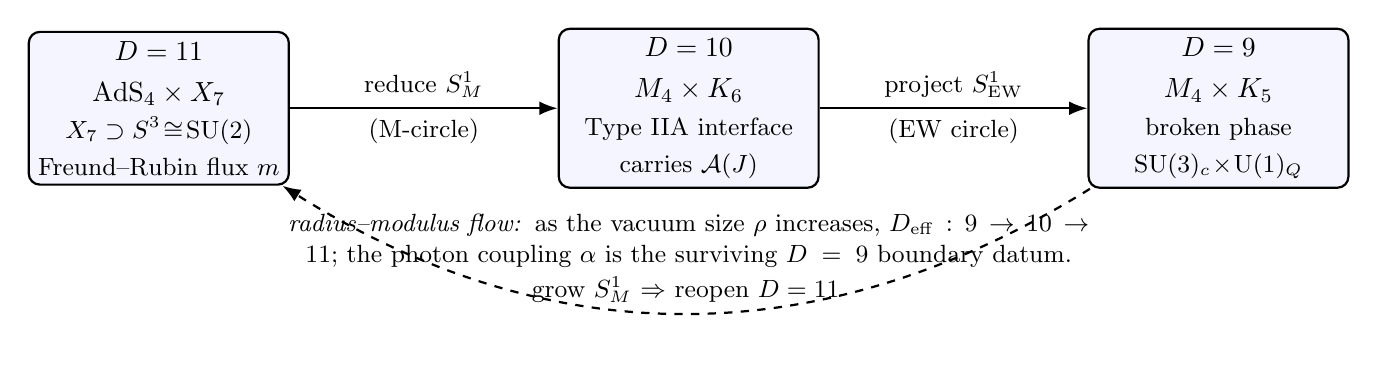
\begin{tikzpicture}[
  box/.style={draw, rounded corners, align=center, minimum width=3.3cm,
    minimum height=1.5cm, thick, fill=blue!4},
  op/.style={->, >=Latex, thick},
  lab/.style={font=\small, align=center}
]
\node[box] (d11) {$D=11$\\[1mm]$\AdS_4\times X_7$\\[0.5mm]\small $X_7\supset S^3\!\cong\!\SU(2)$\\[0.5mm]\small Freund--Rubin flux $m$};
\node[box, right=3.4cm of d11] (d10) {$D=10$\\[1mm]$M_4\times K_6$\\[0.5mm]\small Type IIA interface\\[0.5mm]\small carries $\cA(J)$};
\node[box, right=3.4cm of d10] (d9) {$D=9$\\[1mm]$M_4\times K_5$\\[0.5mm]\small broken phase\\[0.5mm]\small $\SU(3)_c\!\times\!\U(1)_Q$};
\draw[op] (d11) -- node[lab,above]{reduce $S^1_M$}node[lab,below]{(M-circle)} (d10);
\draw[op] (d10) -- node[lab,above]{project $S^1_{\rm EW}$}node[lab,below]{(EW circle)} (d9);
\draw[op, dashed, bend left=32] (d9) to node[lab,above]{grow $S^1_M$ $\Rightarrow$ reopen $D=11$} (d11);
\node[lab, below=0.2cm of d10, text width=11cm]
{\emph{radius--modulus flow:} as the vacuum size $\rho$ increases,
$D_{\rm eff}:9\to10\to11$; the photon coupling $\alpha$ is the surviving
$D=9$ boundary datum.};
\end{tikzpicture}
\caption{The dimensional ladder. Two distinct circle operations connect the
eleven-dimensional Freund--Rubin parent to the nine-dimensional
electroweak endpoint: the M-theory circle $S^1_M$ relates $D=11$ and
$D=10$, while a different electroweak circle $S^1_{\rm EW}$ relates $D=10$
and $D=9$. The electroweak operator $\cA(J)$ lives on the $D=10$ interface
$K_6\supset S^3$.}
\label{fig:ladder}
\end{figure}

\subsection{Probe energy and the $K_5/K_6/K_7$ ladder}
\label{sec:probe}

The cleanest way to read the three ``dimensions'' is not as a change in the
geometry but as a change in the \emph{probe}. The internal geometry is fixed,
with one overall scale; what a given experiment resolves depends on its
energy. A probe of energy $E$ resolves a compact direction of proper radius
$R$ --- excites its Kaluza--Klein tower, whose gap is $1/R$ --- precisely when
\begin{equation}
E\,R\ \gtrsim\ 1,
\label{eq:visibility}
\end{equation}
and is blind to it for $E\,R\ll1$. The internal manifold is built from nested
factors of increasing inverse radius (decreasing size),
\begin{equation}
K_5\ \subset\ K_6=K_5\times S^1_{\rm EW}\ \subset\ K_7=K_6\times S^1_M,
\end{equation}
the electroweak circle $S^1_{\rm EW}$ and the M-theory circle $S^1_M$ being
the two distinct circles of Section~\ref{sec:reduction}. As the probe energy
climbs past the corresponding thresholds $1/R_{\rm EW}$ and $1/R_M$, one
additional internal dimension switches on at each step, so the number of
resolved internal dimensions runs $5\to6\to7$:
\begin{equation}
\boxed{\;
\begin{array}{lllll}
\text{IR probe} & E<1/R_{\rm EW}: & K_5 & D=9 & \SU(3)_c\times\U(1)_Q,\ \text{only }\alpha\ \text{survives};\\[1mm]
\text{EW-scale probe} & 1/R_{\rm EW}<E<1/R_M: & K_6 & D=10 & \text{electroweak }S^3\ \text{resolved, }\cA(J)\ \text{lives here};\\[1mm]
\text{UV probe} & E>1/R_M: & K_7 & D=11 & \text{M-circle open, supergravity parent}.
\end{array}\;}
\end{equation}
Thus the infrared experiment sees a five-dimensional internal space (the
$D=9$ endpoint, where only the electric coupling $\alpha$ is visible); an
experiment at the electroweak scale sees six (the $D=10$ interface carrying
the de Vries operator); and a hypothetical ultraviolet probe sees seven (the
$D=11$ supergravity parent). The ``$9\to10\to11$'' ladder is the
\emph{probe-energy} ordering, not a sequence of distinct theories.

\emph{We live in $D=10$.} The electroweak experiments that measure
$\sinsq$, $M_W$, and $M_Z$ operate at the middle rung: their probe energy
resolves the electroweak $S^3$ but not the M-circle, so the world they see is
ten-dimensional, $M_4\times K_6$, the Type IIA interface on which $\cA(J)$ is
a fluctuation. The eleven-dimensional parent is reached only by a probe above
$1/R_M$ (which we do not have), and the nine-dimensional endpoint only in the
deep infrared after electroweak breaking. The middle rung is not one option
among three; it is our home, and Section~\ref{sec:fermions} shows that it is
also the only rung on which the chiral fermions can live.

This is also the precise meaning of the construction's having one physical
scale. The geometry carries a single overall size (equivalently $\mu$, the
$S^3$ radius, or the flux scale $m$); all dimensionless content --- the spins
$j=0,\half,1$, the flux normalization $c=1$, the charge lattice --- is
topological or representation-theoretic and does not move with that scale.
Different experiments do not change the theory; they change which rungs of
the $K_5\subset K_6\subset K_7$ ladder lie below their resolution.

\subsection{The role of Regge data}

A word on where string Regge dynamics enters, since the relation is sometimes
mistaken for a Regge trajectory. The de Vries positive branch is
\emph{bounded} ($\Xp(J)<1$), whereas a Regge trajectory $M^2\sim J/\alpha'$
is unbounded. They are different objects: the de Vries block is the finite
internal electroweak operator, while the genuine Regge tower is the string
oscillator spectrum that sits \emph{on top} of it,
\begin{equation}
M^2(n,j)=\frac{n-a_0}{\alpha'}+\mu^2\,\Xp\!\bigl(j(j+1)\bigr)
+\Delta M^2_{\rm KK}.
\end{equation}
The string/Regge sector's only role in the electroweak ratio is as a
\emph{selection principle}: it supplies the finite spin set $\{0,\half,1\}$
(Section~\ref{sec:reps}). We are careful to use it \emph{only} for that, and
not for the operator normalization: the level-two truncation fixes which
representations appear, while the off-diagonal coefficient is fixed
independently by the geometric curl ($A_j^\dagger A_j=J$, not the WZW weight
$J/(k+2)$). Treating the finite set $\{0,\half,1\}$ as the electroweak content
(an input, like the gauge group) and the curl as the operator is consistent;
the two statements are logically separate. A direct identification of the de
Vries branch with a Regge trajectory is incorrect and we do not make it.

\subsection{Branches and brane dimension}
\label{sec:branescaling}

There is, however, a clean place where the two branches of $\cA(J)$ meet the
spinning-object literature, and it is worth recording because it organizes the
bounded and unbounded branches into one family. A spinning $q$-brane has the
Regge scaling
\begin{equation}
M^2\ \propto\ J^{\,2q/(q+1)},
\end{equation}
with the three viewpoints: $q=0$ (a point particle / $0$-brane) gives
$M^2\sim J^0=\,$const, a \emph{bounded} spectrum; $q=1$ (the string) gives the
familiar linear trajectory $M^2\sim J$; and $q\to\infty$ (a space-filling
brane) gives $M^2\sim J^2$. The two branches of the de Vries operator sit at
the first two of these endpoints. The positive branch is bounded,
$\Xp(J)\to1$ as $J\to\infty$ --- the $q=0$, point-like behaviour appropriate
to a finite internal (electroweak) operator. The negative branch grows
linearly, $\Xm(J)\to-(J+1)$ --- the $q=1$, string-like behaviour. And the
\emph{branch product},
\begin{equation}
\Xp(J)\,\Xm(J)=-J,
\end{equation}
is exactly the linear (string, $q=1$) Regge invariant: it is the quantity
that scales linearly in the Casimir, while neither branch alone does. The de
Vries block thus packages a point-like (bounded) gauge branch and a
string-like (linear) order-parameter branch into a single operator whose
invariant is the linear trajectory. This is the limited sense in
which Regge structure is present: not as the electroweak spectrum itself, but
as the brane-dimension family whose $q=0$ and $q=1$ endpoints are the two de
Vries branches.

%==============================================================
\section{The electromagnetic coupling at the $D=9$ boundary}
\label{sec:alpha}
%==============================================================

The electroweak ratio is free of continuous moduli (conditional on $c=1$);
the absolute electromagnetic coupling requires one more ingredient, the
absolute size of the surviving $\U(1)_Q$ generator. We collect the standard
Kaluza--Klein normalization and the masslessness of the photon.

\subsection{Couplings from circumferences}

Weinberg's rule~\cite{Weinberg1983} expresses a four-dimensional gauge
coupling in terms of the proper length $L$ of the orbit of the corresponding
internal isometry,
\begin{equation}
g^2=\frac{4\pi^2\kappa^2}{L^2},\qquad \kappa^2=16\pi G,
\end{equation}
with $G$ the four-dimensional Newton constant. For the electroweak
generators $T_3$ and $Y$, with orbit lengths $L_2$ and $L_Y$, the
unbroken couplings are $g_2^2=4\pi^2\kappa^2/L_2^2$ and
$g_Y^2=4\pi^2\kappa^2/L_Y^2$. The weak angle is
$\tan^2\theta_W=g_Y^2/g_2^2=L_2^2/L_Y^2$, and after breaking the
electromagnetic coupling is
\begin{equation}
\frac1{e^2}=\frac1{g_2^2}+\frac1{g_Y^2}
=\frac{L_2^2+L_Y^2}{4\pi^2\kappa^2},
\qquad
\alpha_{\rm EM}=\frac{16\pi^2 G}{L_2^2+L_Y^2}.
\label{eq:alphaweinberg}
\end{equation}
The absence of a cross term $1/g_{2Y}$ in \eqref{eq:alphaweinberg} ---
equivalently $L_Q^2=L_2^2+L_Y^2$ with no $L_{2Y}$ --- is not an assumption
but follows from the structure of the gauge group: there is no
$\mathrm{Ad}$-invariant bilinear form pairing the simple-$\SU(2)$ generator
$T_3$ with the external $\U(1)_Y$, so the gauge-kinetic matrix is diagonal in
the $(T_3,Y)$ basis. The diagonal $\alpha$ formula is therefore exact.

Equation~\eqref{eq:alphaweinberg} shows the division of labour cleanly: the
\emph{ratio} $L_2/L_Y$ is the weak angle (which we obtain from $\cA(J)$,
not from the lengths), while the \emph{absolute} lengths fix $\alpha$.
The de Vries expression \eqref{eq:alpha} is the statement that the same
geometry which fixes the ratio also fixes the combination
$L_2^2+L_Y^2$ that appears in $\alpha$; making this quantitative ---
deriving the absolute $S^3$ and $\U(1)$ radii from the flux $m$ --- is part
of the open problem of the absolute scale.

\subsection{The photon stays massless}

The surviving gauge generator is $Q=T_3+Y$, and the photon's masslessness
is the statement that the order-parameter vacuum is $Q$-neutral. Take the
electroweak doublet basis $\eta_+=\binom10$, $\eta_0=\binom01$ with
$T_a=\tfrac12\sigma_a$, $Y=\tfrac12$. The neutral component satisfies
\begin{equation}
T_3\,\eta_0=-\tfrac12\,\eta_0,\qquad Y\,\eta_0=+\tfrac12\,\eta_0,
\qquad\Longrightarrow\qquad
Q\,\eta_0=(T_3+Y)\,\eta_0=0 .
\label{eq:photon}
\end{equation}
A vacuum $\Phi_0=v_F\,\eta_0$ therefore leaves $\U(1)_Q$ unbroken and the
photon massless --- the $j=0$, $X=0$ slot of $\cA(J)$. The same neutral
vector carries $\SU(2)$ Casimir
$\sum_a\|T_a\eta_0\|^2=\tfrac34=J|_{j=1/2}$, tying the photon-protecting
order parameter to the $j=\half$ branch label.

In the geometry, $\eta_0$ is the $Q$-neutral section of the line bundle
$\cO(1)$ over the weak $\mathbb{CP}^1=S^3/S^1_M$, and the surviving
$\U(1)_Q$ is the diagonal weak--hypercharge frame circle
$P_Q=\ker\chi_N$, with $\chi_N(u_T,u_Y)=u_T^{-1}u_Y$ the neutral character.
We will not need the details; the content is Eq.~\eqref{eq:photon}.

%==============================================================
\section{The negative branch as the Higgs / order parameter}
\label{sec:higgs}
%==============================================================

We promised a reading of the negative branch. The interpretation is forced
by the structure: the $nn$-entry of $\cA(J)$ is a negative mass-squared, the
defining property of an order-parameter (Higgs) direction.

\subsection{The order parameter and $v_{\rm EW}$}

In the broken phase the standard kinetic term of the doublet
$\Phi_0=v_F\eta_0$ gives the gauge masses
\begin{equation}
M_W^2=\tfrac14 g_2^2 v_{\rm EW}^2,\qquad
M_Z^2=\tfrac14(g_2^2+g_Y^2)v_{\rm EW}^2,\qquad
M_\gamma^2=0,
\end{equation}
with $v_{\rm EW}=\sqrt2\,|v_F|$. The de Vries branch fixes the
\emph{ratio} $M_W^2/M_Z^2$; the order-parameter amplitude $v_F$ fixes the
overall scale. Comparing with Eq.~\eqref{eq:massassign},
$\mu^2\Xp(2)=M_Z^2=\tfrac14(g_2^2+g_Y^2)v_{\rm EW}^2$, ties $\mu$ to
$v_{\rm EW}$ and the couplings; numerically $\mu\simeq\sqrt{vM_Z/2}\approx
107\,$GeV, recovering the geometric-mean reading mentioned in (P2). The
identification of the order-parameter modulus with the size modulus
(``Higgs $=$ radion'') is natural in this setting and would make $v_{\rm EW}$
a geometric quantity; we list this as an attractive but unproven option in
Section~\ref{sec:open}.

\subsection{The negative roots and the top/Higgs window}

The magnitudes of the negative roots, with the same single scale, are
\begin{equation}
\mu\sqrt{|\Xm(3/4)|}=122.4\,\text{GeV},\qquad
\mu\sqrt{|\Xm(2)|}=176.2\,\text{GeV}.
\end{equation}
The proximity to $m_H=125.25\,$GeV and $m_t=172.7\,$GeV is suggestive, and
it sharpens under the complex-pole reading of the relation (where the
masses are real parts of complex poles). We stress that this is a
\emph{diagnostic}: we have not derived the identification of the negative
$j=\half$ root with the Higgs scalar or the negative $j=1$ root with the
top quark. But the fact that one scale $\mu$, fixed by $M_Z$, simultaneously
places the positive branch on $(M_W,M_Z)$ and the negative branch near
$(m_H,m_t)$ is part of what makes the relation hard to dismiss as a single
accident. It is also exactly the pattern one expects if all four masses are
the four roots of two copies of one quadratic --- the deepest version of
the de Vries claim, and the one most worth testing. It is suggestive that the
negative-branch point $(m_t,m_H)\approx(176,122)\,$GeV lies in the same
near-critical region of the Standard Model $(m_t,m_H)$ plane mapped out by the
vacuum-stability analyses~\cite{Buttazzo2013}, an entirely independent
calculation that knows nothing of $\cA(J)$; we record this as a coincidence
worth watching, not as evidence.

\subsection{The Higgs mass as a curvature}

The Higgs mass is, in this language, the radial curvature of the
order-parameter potential at its minimum,
\begin{equation}
M_H^2=\frac1{Z_H}\frac{\partial^2 V_{\rm eff}}{\partial h^2}\bigg|_{*},
\end{equation}
with $Z_H$ the kinetic normalization of the radial mode $h$. Deriving
$V_{\rm eff}$ from the flux compactification --- and hence $M_H$ and $v$
from the same data that give $M_W/M_Z$ --- is the scalar-sector analogue of
the flux-coefficient problem \eqref{eq:conehypothesis}. We do not solve it;
we note that the negative-branch value $122.4\,$GeV is the target.

\subsection{Higgs as radion}
\label{sec:radion}

The most economical scenario identifies the order-parameter modulus with the
size modulus of the internal geometry --- the Higgs field is the radion of
the electroweak $S^3$. This is attractive for three reasons. First, it
removes a field: the same modulus that stabilizes the compactification and
the field that breaks electroweak symmetry are one and the same, so no
separate Higgs sector need be postulated. Second, it explains the
``geometric mean'' value of the mixing scale: if $v_{\rm EW}$ and $M_Z$ are
both functions of the single radion, the natural electroweak scale is their
geometric mean $\mu\sim\sqrt{v\,M_Z/2}\approx107\,$GeV, exactly the value
extracted in (P2). Third, it makes the Higgs couplings predictions rather
than inputs: a radion Higgs has definite, generically non-standard couplings
$g_{hWW},g_{hZZ},g_{hff}$, providing a falsifiable coupling-pattern test.
Precedents for ``Higgs as a geometric modulus'' in extra-dimensional models
are well known, and the present setting --- a relevant order-parameter
direction of the de Vries block whose condensation is breaking --- is a
natural home for the idea. We list it as the preferred but unproven scenario
for the absolute scale.

\subsection{The two-sheet (finite-distance) reading}
\label{sec:connes}

There is a complementary, useful language for the order parameter, due in
spirit to Connes's noncommutative-geometry picture of the Standard Model.
The neutral section $\eta_0\in H^0(\mathbb{CP}^1,\cO(1))$ that protects the
photon (Section~\ref{sec:alpha}) can be read as a connection in a
\emph{finite} (two-point) extra direction --- two ``sheets'' separated by a
distance set by the inverse order-parameter amplitude,
\begin{equation}
\ell_H=\frac1{\|\Phi_0\|}=\frac{\sqrt2}{v_{\rm EW}}.
\end{equation}
In this reading the electroweak scale is literally a distance --- the gap
between the sheets --- and the Higgs mass is the curvature of the
finite-direction potential.

This reading does more than provide a picture: it is a \emph{limit of the
construction that avoids the Kaluza--Klein tower}. The objection to any
$S^3$-based electroweak sector is the infinite tower $j=0,\half,1,\tfrac32,
\dots$ (Section~\ref{sec:towervsdoublet}); one wants only the finite set
$\{0,\half,1\}$. The Connes limit supplies exactly that. As the weak
$\mathbb{CP}^1$ (equivalently the Hopf $S^3$) is taken to a degenerate,
finite-distance configuration, the internal geometry collapses to a
\emph{finite spectral triple} --- a finite-dimensional algebra with a
finite Dirac operator --- whose spectrum is a finite set rather than a tower.
In that limit the off-diagonal curl $\star\dd$ becomes a finite matrix (the
finite-direction Dirac operator), and the de Vries block $\cA(J)$ is its
fluctuation Hessian, with the photon, $W$, and $Z$ the entire spectrum and no
heavy partners at all. The Connes (finite spectral triple) limit is therefore
the tower-free face of the same construction: where the geometric description
(Section~\ref{sec:geometry}) realizes $\{0,\half,1\}$ as the lowest rungs of a
tower, the noncommutative limit realizes them as the \emph{complete} spectrum
of a finite internal space. The two are continuously connected by shrinking
the weak circle, and the electroweak block is the common content. Making the
limit precise --- and showing the de Vries block is the spectral-action
fluctuation Hessian of the finite triple --- is open; we record it because it
removes the tower objection at the cost of replacing the smooth $S^3$ by its
finite (noncommutative) degeneration.

\subsection{Rigidity: why the model cannot reach $M_W=M_Z$}
\label{sec:rigidity}

A natural objection to any single-operator account of $W$ and $Z$ is that it
might collapse the two into one. The de Vries block answers this cleanly:
$M_W=M_Z$ would require $\Xp(3/4)=\Xp(2)$, i.e.\ $\tfrac34=2$, which is
false; the two masses are \emph{rigidly} separated because $j=\half$ and
$j=1$ are different representations. Equivalently, in the
$g$-language, $M_W=M_Z$ needs $g_Y=0$, and the de Vries structure forbids it
because the hypercharge mixing is locked to the $j=1$ Casimir. This rigidity
is a feature, not a bug: it is the statement that the weak angle is a fixed
number, and it is the reason the relation is falsifiable. The separation
$M_W<M_Z$ (rather than the reverse) follows from the monotonicity of
$\Xp(J)$ and the ordering $j_W=\half<j_Z=1$ --- the lighter gauge boson sits
on the lower internal representation.

%==============================================================
\section{Relation to other pictures of electroweak symmetry breaking}
\label{sec:other}
%==============================================================

The branch operator $\cA(J)$ is an unusual way to organize electroweak mass
generation, and it is worth situating it among the standard pictures, both
to clarify what is new and to inherit their constraints.

\subsection{Custodial symmetry and $\rho=1$}

Any account of $W$ and $Z$ masses must respect the custodial
$\SU(2)$ that protects the tree-level relation
$\rho\equiv M_W^2/(M_Z^2\cos^2\theta_W)=1$. In the de Vries assignment this
is automatic: with $M_W^2=\mu^2\Xp(3/4)$, $M_Z^2=\mu^2\Xp(2)$, and
$\cos^2\theta_W=\Xp(3/4)/\Xp(2)$ by construction \eqref{eq:ratio}, one has
\begin{equation}
\rho=\frac{M_W^2}{M_Z^2\cos^2\theta_W}
=\frac{\Xp(3/4)}{\Xp(2)\cdot\Xp(3/4)/\Xp(2)}=1
\end{equation}
identically. The relation $\rho=1$ is thus not an extra input but a
consistency property of defining the weak angle through the same operator
that gives the masses. This is reassuring: a generic two-channel mass mixing
would violate $\rho=1$ and be excluded by precision data at the per-mille
level; the de Vries structure passes because $\cos^2\theta_W$ is
\emph{defined} as the mass ratio.

\subsection{Higgsless and boundary-condition breaking}

The resolvent form of $\cA(J)$ (Appendix~\ref{app:algebra}),
$X=J/(J+X)$, is the hallmark of \emph{boundary-condition} electroweak
breaking, as in five-dimensional Higgsless and gauge-Higgs unification
models: there, gauge-boson masses are the zeros of a transcendental
function obtained by imposing boundary conditions at the ends of an
interval, and the lightest modes solve a one-pole relation of exactly this
type. The de Vries block is the minimal, two-channel truncation of such a
boundary problem, with the ``interval'' being the radial direction of the
electroweak $S^3$ and the boundary condition being the order-parameter
vacuum. This connection is encouraging on two counts: boundary-condition
models are known to give $\rho=1$ and acceptable precision-electroweak fits
when custodial symmetry is built in, and they realize the off-diagonal
mixing as a genuine geometric (Kaluza--Klein) effect rather than a Yukawa
coupling. The de Vries relation can be read as the statement that the
electroweak interval is the round $S^3$, whose boundary spectrum is fixed by
$\SU(2)$ representation theory.

\subsection{Magnetic-dual and partially composite readings}

The appearance of the negative branch as an order parameter invites a
magnetic-dual reading: $j=\half$ may label an electric (or dual) variable
whose $W$ is a magnetic/IR pole, with $W$ and $Z$ partially composite. In
such Seiberg-dual or partially composite scenarios the two-vector content
($W$ as a magnetic pole, the elementary gauge field as the electric one) is
the resolution of the apparent puzzle that one $\SU(2)$ representation must
furnish two physical vectors. We do not commit to this reading --- it
requires a strongly coupled dual we have not constructed --- but it is the
natural language for ``the de Vries block maps one internal representation
into a gauge pole and an order-parameter pole,'' and it connects the
construction to the well-developed literature on composite and dual
electroweak sectors. The branch product $\Xp\Xm=-J$ is the dual-pair
invariant in this language.

\subsection{The seesaw analogy}

Finally, the structure $X^2+JX-J=0$ is formally a seesaw: a light state
($\Xp\to\sqrt J$ for small $J$, $\Xp\to1$ for large $J$) and a heavy state
($\Xm\to-(J+1)$ for large $J$) mixing through an off-diagonal $\sqrt J$, with
the product of masses fixed to $-J$. The familiar neutrino seesaw has a
\emph{constant} heavy scale; here the ``heavy'' scale is the
$J$-dependent order-parameter mass, and the off-diagonal is the
$J$-dependent curl mixing, so the two are locked. In terms of the physical
mass-squares $M_\pm^2=\mu^2 X_\pm(J)$ (with $M_-^2<0$ the order-parameter
mass) the reciprocal relation reads
\begin{equation}
\frac1{M_+^2}+\frac1{M_-^2}
=\frac1{\mu^2}\,\frac{X_+ + X_-}{X_+ X_-}
=\frac1{\mu^2}\,\frac{-J}{-J}=\frac1{\mu^2},
\end{equation}
the inverted (parallel-resistance) form of the relation, and another way to
see that the two branches are the two roots of one structure rather than
independent objects.

%==============================================================
\section{Global form and the charge lattice}
\label{sec:globalform}
%==============================================================

A brief, standard, and genuinely derivable piece: the global form of the
gauge group along the ladder. The unbroken Standard Model gauge group is
\begin{equation}
G_{\rm SM}=\frac{\SU(3)_c\times\SU(2)_L\times\U(1)_Y}{\Z_6},
\qquad y=6Y,
\end{equation}
the $\Z_6$ being generated by
$\zeta_6=(\omega_3,-1,e^{i\pi/3})$ with $\omega_3=e^{2\pi i/3}$. On a state
of colour triality $t$, weak weight $T_3=m$, and charge $Q=m+Y$,
\begin{equation}
\zeta_6:\ \omega_3^{t}\,e^{2\pi i m}\,e^{i\pi y/3}
=\omega_3^{t}\,e^{2\pi i Q}
=\omega_3^{t}\,e^{2\pi i q_3/3},\qquad q_3=3Q,
\end{equation}
so after electroweak breaking the surviving identification is
$\zeta_6\mapsto\zeta_3=(\omega_3,e^{2\pi i/3})$ with $\zeta_3^3=1$, and the
$D=9$ endpoint group is
\begin{equation}
G_{D9}=\frac{\SU(3)_c\times\U(1)_Q}{\Z_3}.
\end{equation}
This $\Z_6\to\Z_3$ descent is the global-form content of the ladder; in the
geometry it is carried by the diagonal line bundle
$c_1(L_N)=c_1(L_Y)-c_1(L_{T_3})$ of the neutral character $\chi_N$. It is
the one part of the ``$M^{pqr}$ package'' that survives our critique below
intact, because it is topology, not a fit.

%==============================================================
\section{Fermions, chirality, and why we live in $D=10$}
\label{sec:fermions}
%==============================================================

The construction so far concerns the electroweak \emph{bosons}: the gauge
fields from isometries and the mass operator $\cA(J)$ from flux. The fermions
force a sharpening of the whole picture, and that sharpening is the deepest
structural statement of the paper: \emph{we live in $D=10$.} The
eleven-dimensional supergravity is only the ultraviolet parent; the
nine-dimensional endpoint is only the infrared limit; the physics we measure
--- including the chiral fermions --- lives at the ten-dimensional, Type IIA
string interface $K_6$. The chirality problem is what makes this unavoidable.

\subsection{The chirality obstruction in $D=11$}

The fermions of the Standard Model are chiral: left- and right-handed
components transform differently under $\SU(2)_L\times\U(1)_Y$. Witten's
theorem~\cite{Witten1981} is that one \emph{cannot} obtain a chiral
four-dimensional spectrum from the Kaluza--Klein reduction of eleven-dimensional
supergravity on a \emph{smooth} compact seven-manifold: the four-dimensional
massless fermions are the zero modes of the internal Dirac operator
$\slashed D_K$, their net chirality is the index $\mathrm{ind}\,\slashed D_K$,
and on a smooth boundaryless homogeneous space of the $M^{pqr}$ type this
index does not deliver chiral generations --- left and right modes pair up.
This is the single most serious reason the classical eleven-dimensional
Kaluza--Klein program of the early 1980s did not become the Standard Model. It
is an obstruction of the \emph{smooth $D=11$ reduction}, and it is sharp.

\subsection{Why the boson result is unaffected}

The obstruction does not touch the electroweak boson result, and it is worth
saying why before resolving it. The mass operator $\cA(J)$ lives in the
\emph{bosonic} fluctuation spectrum --- the metric, the three-form, and their
flux mixing on the $S^3$ factor --- governed by the Laplacian and the curl,
not by the Dirac index. The weak mixing angle is a statement about how the
gauge bosons distribute over internal $\SU(2)$ representations, insensitive to
the fermion sector, exactly as the gauge group itself is an isometry statement
independent of the fermions. The boson prediction $\sinsq=0.2231$ therefore
stands on its own.

\subsection{We live in $D=10$: chirality from branes}

The resolution of the chirality obstruction is not to deform the smooth
eleven-dimensional reduction but to recognize that the theory we actually
inhabit is \emph{ten}-dimensional. Reducing eleven-dimensional supergravity on
the M-theory circle $S^1_M$ gives Type IIA string theory in $D=10$, and Type
IIA has an ingredient that smooth supergravity lacks: \emph{D-branes}. Chiral
fermions are then routine. They arise as open-string zero modes at the
intersections of D-branes, or equivalently from D-branes wrapping cycles at
ADE singularities, with the net chirality given by a topological
intersection number rather than by the (vanishing) smooth Dirac index. This is
the standard, and successful, string route to the chiral Standard Model:
intersecting-brane and brane-at-singularity constructions in Type II string
theory. In our setting the relevant branes are the D-branes wrapping the
electroweak $K_6=$ ($S^3\cong\SU(2)$ sector) and the colour/hypercharge
cycles, with chiral matter localized at their intersections.

The eleven-dimensional and ten-dimensional pictures are the two faces of one
structure, related by the M-circle of Section~\ref{sec:probe}. The chiral
matter that appears in $D=10$ at brane intersections lifts, in the $D=11$
M-theory limit, to the Acharya--Witten mechanism~\cite{AcharyaWitten2001}:
chiral fermions at codimension-seven conical singularities of a
$G_2$-holonomy space, where D6-branes become loci of ADE singularity. The two
descriptions agree, but the \emph{physical, weakly coupled} description --- the
one in which both the de Vries boson operator and the chiral fermions are
simultaneously visible and computable --- is the ten-dimensional one. This is
the precise content of ``we live in $D=10$'':
\begin{itemize}
\item $D=11$ (the smooth $M^{pqr}$ parent, $K_7$) is the ultraviolet
completion; it gives the isometries (the gauge group) and the Freund--Rubin
flux, but \emph{cannot}, while smooth, give chiral fermions;
\item $D=10$ (Type IIA on $M_4\times K_6$, $K_6\supset S^3$) is where we live;
it carries the de Vries operator $\cA(J)$ \emph{and}, through its D-branes,
the chiral fermions, the Yukawa couplings, and the flavour structure;
\item $D=9$ ($K_5$) is the infrared endpoint after electroweak breaking, where
only $\SU(3)_c\times\U(1)_Q$ and the coupling $\alpha$ survive.
\end{itemize}
The de Vries relation is thus a \emph{ten-dimensional} statement: the
electroweak operator is a fluctuation of the Type IIA interface, and the same
ten-dimensional frame is the one in which chirality is solved. We do not
construct the explicit brane configuration that yields three generations, the
Yukawas, and the CKM matrix; that is the frontier. What the chirality problem
establishes is the \emph{location} of the physics --- $D=10$ --- and that
location is exactly where the de Vries operator was found.

\subsection{Chirality across the ladder: why only $D=10$ is delicate}

The three rungs stand in a clarifying relation to chirality, and it is the
relation that fixes $D=10$ as the home of the fermions just as it is the home
of $\cA(J)$.
\begin{itemize}
\item \textbf{$D=11$: chirality fails.} The smooth eleven-dimensional
reduction cannot produce chiral fermions (Witten's no-go). But we do not live
there: $D=11$ is the ultraviolet M-theory parent, reached only above the
M-circle threshold.
\item \textbf{$D=10$: chirality is realized, and is the whole point.} The
electroweak group $\SU(2)_L\times\U(1)_Y$ is \emph{chiral} --- left- and
right-handed fermions carry different charges --- and this chiral structure is
an electroweak, i.e.\ ten-dimensional, phenomenon. It is realized by the
D-branes of the Type IIA interface, whose open-string intersection modes are
chiral. Chirality is delicate here, and here it is
solved.
\item \textbf{$D=9$: chirality does not even arise.} After electroweak
breaking the surviving group is $\SU(3)_c\times\U(1)_Q$ --- QCD plus
electromagnetism --- which is \emph{vector-like}: left- and right-handed
fields carry identical colour and electric charges, so the fermions are
ordinary Dirac (vector) fermions and no chiral index need be non-zero. The
infrared endpoint therefore has \emph{no} chirality problem to fail; there is
nothing to obstruct.
\end{itemize}
The pattern is that chirality is born and resolved together, at the middle
rung. It is absent in the infrared (the residual group is vector), impossible
in the smooth ultraviolet (the no-go), and exactly realized in between, in the
ten-dimensional electroweak world where the weak interaction is chiral and the
de Vries operator lives. That the same rung carries both the parity-violating
fermions and the boson mass relation is, we think, the strongest structural
reason to read the de Vries relation as a statement about $D=10$.

Each ingredient of this argument is standard: the impossibility of chiral
fermions from smooth eleven-dimensional reduction is Witten's
theorem~\cite{Witten1981}; the appearance of chiral matter from D-branes is
the basis of string phenomenology; and the vector-like character of QCD plus
electromagnetism is elementary. What is perhaps not standard is the
synthesis --- that these three facts \emph{together} pin the physical,
chirality-bearing rung to $D=10$, with both neighbours chirality-trivial for
opposite reasons --- and that this is the same rung on which the electroweak
boson mass ratio is geometric. The argument uses nothing beyond textbook
results, which is a point in its favour: a robust conclusion should follow
from robust inputs.

\subsection{A remark on the global form and the lattice}

The charge-lattice and global-form data of Section~\ref{sec:globalform} are
the bridge between the two sectors. The $\Z_6$ identification, the
hypercharge normalization $y=6Y$, and the descent to $\Z_3$ are exactly the
data that a consistent chiral spectrum must respect, and they are carried by
the same line bundles over the weak $\mathbb{CP}^1$ that furnish the boson
slots $j=0,\half,1$. That the boson construction already fixes the global form
to be the one compatible with Standard Model hypercharges is a nontrivial
consistency check, and a hint that the singular completion, when built, will
find the charge lattice waiting for it.

%==============================================================
\section{The $M^{pqr}$ coupling-ratio program and the over-determination of the weak angle}
\label{sec:control}
%==============================================================

The classical Kaluza--Klein literature suggests a different, tempting route
to the weak angle --- directly from the $M^{pqr}$ orbit lengths --- and it is
important to establish quantitatively why that route does not predict the
angle, and why we obtain it instead from $\cA(J)$.

\subsection{The Bailin--Love coupling ratios}

Weinberg~\cite{Weinberg1983} and Bailin and Love~\cite{BailinLove1984,BailinLove1987}
computed the gauge-coupling ratios on $M^{pqr}$ via the orbit-length rule
\eqref{eq:weinbergrule}. The weak-to-hypercharge ratio is a definite
function of the integer labels $(p,q,r,n)$ and the Einstein shape parameter
$\beta$ fixed by $q/p$,
\begin{equation}
4\beta^3-6\beta^2+\Bigl(\tfrac94+\tfrac{q^2}{p^2}\Bigr)\beta
-\tfrac12\tfrac{q^2}{p^2}=0\ \ (0<\beta<\tfrac12),
\qquad
\frac{g_Y^2}{g_2^2}=\frac32\frac{p^2n^2}{r^2}\,
\frac{(3-4\beta)^2(1+\beta)}{1-2\beta}
\equiv F\!\Bigl(\tfrac qp\Bigr)\frac{p^2n^2}{r^2}.
\label{eq:bailinlove}
\end{equation}
The structure is a continuous function $F(q/p)$ of the shape, multiplied by
the rational $p^2n^2/r^2$ from the integer winding and charge-normalization
data.

\subsection{The integer fit}

Scanning \eqref{eq:bailinlove} for the de Vries value, the labels
$(p,q,r,n)=(12,14,91,1)$ give $\beta=0.328481702\ldots$ and
\begin{equation}
\frac{g_Y^2}{g_2^2}\Big|_{(12,14,91,1)}=0.2871699126,
\qquad
\tan^2\theta_{\rm dV}=0.2871691363,
\end{equation}
a match to a relative $2.7\times10^{-6}$. Taken at face value this looks like
a six-digit prediction. It is not, for the reason we now make quantitative.

\subsection{Over-determination: the family is dense around the target}
\label{sec:overdet}

The map $(p,q,r,n)\mapsto F(q/p)\,p^2n^2/r^2$ has four integer inputs
constrained by one measurement, $\sinsq$, itself known only to $\sim10^{-3}$.
For any fixed shape $q/p$ the residual factor $(np/r)^2$ ranges over the
\emph{squares of the positive rationals}, which are dense in $\R_{>0}$; layering
the continuous variation of $F(q/p)$ over Farey fractions $q/p$ makes the
achievable set dense around the target. A direct scan over modest integers
($p,q\le30$, $r\le300$, $n\le3$) bears this out: there are $138$ distinct
geometries reproducing the measured weak angle to within experimental error
($10^{-3}$), $12$ matching to $10^{-4}$, and $2$ to $10^{-5}$. A representative
sample of \emph{independent} geometries (distinct $\beta$, not rescalings) is
given in Table~\ref{tab:overdet}; every row reproduces $\tan^2\theta_{\rm dV}$
better than experiment can resolve.
\begin{table}[h]
\centering
\begin{tabular}{cccccc}
\toprule
$(p,q,r,n)$ & $q/p$ & $\beta$ & $g_Y^2/g_2^2$ & rel.\ dev.\\
\midrule
$(12,14,91,1)$ & $1.1667$ & $0.328482$ & $0.2871699$ & $2.7\times10^{-6}$\\
$(7,26,293,2)$ & $3.7143$ & $0.490419$ & $0.2871666$ & $8.8\times10^{-6}$\\
$(11,11,159,2)$ & $1.0000$ & $0.250000$ & $0.2871722$ & $1.1\times10^{-5}$\\
$(14,21,125,1)$ & $1.5000$ & $0.418130$ & $0.2871736$ & $1.6\times10^{-5}$\\
$(22,25,165,1)$ & $1.1364$ & $0.315495$ & $0.2871638$ & $1.9\times10^{-5}$\\
$(11,5,76,1)$ & $0.4545$ & $0.047357$ & $0.2871758$ & $2.3\times10^{-5}$\\
\bottomrule
\end{tabular}
\caption{Independent $M^{pqr}$ geometries reproducing the de Vries weak angle.
Each has a distinct Einstein shape $\beta$; all match the measured value to
better than experimental precision. The advertised $(12,14,91,1)$ is one of
many, and its $2.7\times10^{-6}$ deviation is finer than the data warrant. The
match is a property of the density of the family, not a selection of the
manifold.}
\label{tab:overdet}
\end{table}

A datum of relative precision $\delta\sim10^{-3}$ can carry at most
$\sim\ln(\text{range}/\delta)$ of selection information; the pre-image of the
$\delta$-ball around the target contains $O(10^2)$ integer tuples already in
the smallest scan and diverges as the cutoffs grow. The likelihood that the
Standard Model ``selects'' $(12,14,91,1)$ rather than one of its competitors
is therefore $\lesssim1/138$: the integer match is a fit, not a prediction.

\subsection{Consequence for the present construction}

Accordingly the weak angle in this paper is \emph{not} taken from
\eqref{eq:bailinlove}. It is taken from the parameter-free representation
theory of $\cA(J)$ (Corollary~\ref{cor:angle}), whose only inputs are the
spins $j=\half,1$ and the flux normalization $c=1$ --- a single statement
\eqref{eq:conehypothesis}, not a four-integer search. The $M^{pqr}$ geometry
enters only as the $D=11$ grow-limit of the minimal $K_6$
(Section~\ref{sec:k6}), through its isometries (the gauge group), its
topology, and its charge lattice
(Section~\ref{sec:globalform}); its orbit lengths fix the absolute scale of
$\alpha$ through \eqref{eq:weinbergangle} but not the angle. The methodological
discussion of why integer fits of this kind are to be avoided is collected in
Appendix~\ref{app:llm}.

%==============================================================
\section{Predictions and falsifiability}
\label{sec:predictions}
%==============================================================

A physical theory earns its keep by making falsifiable statements. Here are
the ones that follow from the construction.

\paragraph{(F1) The weak angle is a fixed number.}
$\sinsq=0.22310$, on-shell, with no scale or scheme freedom in the ratio.
This already agrees with experiment to $2\times10^{-4}$. Any future shift of
the measured on-shell value by more than $\sim10^{-3}$ would falsify the
$c=1$ form (cf.\ Table~\ref{tab:cscan}).

\paragraph{(F2) A neutral spin-zero state near $96.5\,$GeV.}
This prediction is conditional on the truncation mechanism. In the
\emph{physical-tower} (energetic) reading, the $j=\tfrac32$ rung is a heavy
but real state, a $Q$-neutral scalar at
$M_{3/2}=\mu\sqrt{\Xp(15/4)}=96.5\,$GeV --- intriguingly close to the
persistent $\sim95$--$96\,$GeV excesses in light-Higgs searches. In the
\emph{finite} (level-two / Connes, Section~\ref{sec:connes}) reading the
spectrum is exactly $\{0,\tfrac12,1\}$ and there is no such state. The two
readings are thus distinguished by the presence or absence of the $96.5\,$GeV
scalar: its discovery would select the physical tower, its exclusion the
finite internal geometry.

\paragraph{(F3) The two-spin tower.}
The relation generalizes to any pair of internal spins,
\begin{equation}
\sin^2\theta(j_a,j_b)=1-\frac{\Xp(J_a)}{\Xp(J_b)},
\qquad J_i=j_i(j_i+1),
\end{equation}
with the electroweak case $(j_a,j_b)=(\half,1)$. Sample values:
$\sin^2\theta(\half,\tfrac32)=0.307$,
$\sin^2\theta(1,\tfrac32)=0.108$,
$\sin^2\theta(\half,2)=0.349$. If any further gauge or scalar splitting in
an extended sector follows this family, it is a direct signature of the same
operator.

\paragraph{(F4) The negative branch.}
The model predicts that the Higgs and top masses are the negative-branch
partners of the $W$ and $Z$, $m_H\approx\mu\sqrt{|\Xm(3/4)|}=122\,$GeV and
$m_t\approx\mu\sqrt{|\Xm(2)|}=176\,$GeV. The pattern is testable as
precision on $m_t$, $m_H$, and the pole-mass definitions improves; the
relevant comparison is to the pole (not $\overline{\rm MS}$) masses and to
the vacuum-stability boundary.

\paragraph{(F5) No tuned weak-angle integers.}
A specific \emph{negative} prediction: the correct theory does \emph{not}
select $\sinsq$ by an $M^{pqr}$-type integer fit. If a first-principles
derivation of the labels $(p,q,r,n)=(12,14,91,1)$ from a dynamical
principle were ever produced, it would be in tension with the present claim
that the angle comes parameter-free from $\cA(J)$ with $c=1$. The two
routes predict the \emph{same} number but have different theoretical
content, and they are distinguishable by whether the absolute coupling
$\alpha$ and the $j=\tfrac32$ state come out right.

%==============================================================
\section{Open problems}
\label{sec:open}
%==============================================================

We list the genuine gaps, in decreasing order of importance, so that the
status of the program is unambiguous.

\begin{enumerate}
\item \textbf{The flux coefficient $c=1$, and three residues.}
Proposition~\ref{prop:cone} reduces ``compute $c$'' to the single-portal
condition, and Section~\ref{sec:ghu} identifies that condition with
gauge--Higgs unification (the Higgs as the internal weak gauge component).
Gauge--Higgs unification \emph{derives} the bare-Casimir normalization ---
because the portal is the algebraic gauge current $T_a$ (Casimir $J$), not the
curvature-shifted curl --- and supplies a natural home for a flat,
single-portal Higgs; it does \emph{not}, on its own, produce the indefinite
Schur block (the standard $S^2$ gauge--Higgs spectrum is a Goldstone with
$\sqrt J$ mixing plus a separate scalar of mass $J$). Three sharp residues
remain: \emph{(a)} the single-portal/Schur identification (that the Goldstone
mixing and the scalar mass are one operator's completion); \emph{(b)} the
Hosotani coefficient (that the magnitude of the negative diagonal is exactly
$-A_jA_j^\dagger$, from the flux/loop potential on the weak
$\mathbb{CP}^1/S^3$); and \emph{(c)} the pole identification (that the $W,Z$
masses are the Schur eigenvalues, the mass-ratio reading giving $0.2231$,
rather than the embedding coupling ratio giving the textbook $\tfrac14$).
Each is a definite, answer-blind computation, and together they are the most
important open problem.
\item \textbf{The absolute scale.} The relation fixes ratios; one
dimensionful input ($\mu$, or the $S^3$ radius, or $v_{\rm EW}$) remains.
Tying $\mu$ to the flux $m$ and ultimately to the Planck scale --- and in
particular deriving the absolute orbit lengths $L_2,L_Y$ that fix $\alpha$
through \eqref{eq:alphaweinberg} --- is open. We recall the cautionary
result of Ezawa and Koh~\cite{EzawaKoh1984}, who found that the raw
$\SU(3)\times\SU(2)\times\U(1)$ couplings of the unbroken
eleven-dimensional compactification come out far from the observed
strengths; this is consistent with our position that the absolute scale (and
the running to it) is unresolved, even though the \emph{ratio} that gives the
weak angle is not. The ``Higgs $=$ radion'' identification, if correct,
would make $v_{\rm EW}$ geometric.
\item \textbf{The renormalization scheme of $\sinsq$.} The predicted
$0.22310$ is the \emph{on-shell} angle $1-M_W^2/M_Z^2$, and it should be
compared only to the on-shell value $0.22305(20)$, not to the
$\overline{\rm MS}$ coupling angle $\hat s_Z^2\simeq0.23122$. A geometric
construction of \emph{couplings} would more naturally yield an
$\overline{\rm MS}$-like quantity; that ours lands on the on-shell mass ratio
reflects that $\cA(J)$ is a mass operator, not a coupling operator. Making
the scheme assignment precise --- and likewise placing the
$1/\alpha=135.3$ of \eqref{eq:alpha} on a definite scale between
$\alpha(0)^{-1}=137.036$ and $\alpha(M_Z)^{-1}\approx128$ --- is open.
\item \textbf{The vacuum: cosmological constant and $\AdS_4$ versus
Minkowski.} The Freund--Rubin limit is an $\AdS_4$ vacuum, whereas the
observed four-dimensional spacetime is nearly Minkowski. Uplifting to a small
or zero cosmological constant, and confirming that the electroweak block
survives the uplift, is an unaddressed standard problem; we have used $\AdS_4$
only as the controlled setting in which the flux spectrum is known.
\item \textbf{Moduli stabilization.} The construction carries at least the
overall scale $\rho$ and the shape modulus $\lambda$. We have argued that
$\lambda$ plays the role of the order parameter (Higgs/radion), but we have
not exhibited a stabilizing potential that fixes $\rho$ and gives $\lambda$
the tachyonic curvature $-J$ with the right coefficient; this is the same
computation as the $c=1$ problem viewed in the moduli potential.
\item \textbf{Spin structure for fermions.} $\mathbb{CP}^2$ is not spin; it is
spin$^{c}$. Any fermion construction on $K_6$ must use the spin$^c$
structure (a $\U(1)$ gauge bundle tensored with the spinors), which is in
fact natural here because the hypercharge line bundle supplies exactly such a
$\U(1)$. We note this as a constraint the (deferred) fermion sector must
respect, not as a difficulty for the boson result.
\item \textbf{Chiral fermions and generations.} We have computed the
electroweak \emph{boson} sector. Chiral fermions, three generations, the
Yukawa/CKM structure, and the strong sector are untouched and are the hard
core of any realistic Kaluza--Klein program; the classical no-go theorems on
chirality from smooth compactification~\cite{Witten1981} apply and likely
force a singular ($G_2$/ADE) refinement of $X_7$.
\item \textbf{The branch/orbit normalization subtlety.} The $j=\half$
Casimir is $\tfrac34$, while the literal charged-Higgs orbit norm
$\|T_+H_0\|^2/\|H_0\|^2$ is $1$. Both are correct statements about the same
doublet; the de Vries spectrum uses the Casimir $\tfrac34$ as the branch
label, and the map to the physical $W$-pole normalization is a real
conceptual point that deserves a cleaner treatment than we have given.
\item \textbf{A rigorous $X_7$.} We kept $X_7$ schematic. Specifying a
concrete Freund--Rubin seven-manifold that (a) contains the electroweak
$S^3\cong\SU(2)$ at the self-dual point, (b) carries colour and hypercharge
with the right charge lattice, and (c) admits the chiral refinement of
point (4), is the geometric completion of the program.
\end{enumerate}

%==============================================================
\section{Conclusions}
\label{sec:conclusion}
%==============================================================

We began with an arithmetic fact: the on-shell weak mixing angle and the
$W/Z$ mass ratio are reproduced, with no free parameter, by the positive
eigenvalue of a $2\times2$ matrix $\cA(J)$ evaluated at the $\SU(2)$
Casimirs of $j=\half$ and $j=1$. We have argued that this fact is the
shadow of a Kaluza--Klein theory of a very classical kind. The pieces fit
together with little slack:
\begin{itemize}
\item the diagonal Casimir $J=j(j+1)$ is one quarter of the scalar
Laplacian on an internal $S^3\cong\SU(2)$, and the half-integer $j=\half$ is
the Peter--Weyl fingerprint of the group manifold rather than its $\SO(3)$
quotient;
\item the off-diagonal $\sqrt J$ is the matrix element of the curl
$\star\dd$, a first-order, unit-normalized, self-adjoint operator whose
square is the Laplacian --- which is also why the electroweak masses are a
bounded doublet rather than an unbounded tower;
\item the negative diagonal $-J$ is the form-degree mixing induced by the
$D=10$ Type IIA background flux on $K_6$, and the coefficient $c=1$ is
\emph{conditionally derived} (Proposition~\ref{prop:cone}): it is forced when
the order parameter is a single-portal flat modulus, which
Section~\ref{sec:ghu} identifies with gauge--Higgs unification --- the Higgs
as the internal weak gauge component --- whose gauge-current (not metric-curl)
portal \emph{derives the bare-Casimir normalization}, the distinction that
separates $0.223$ from the curvature-shifted alternatives, while the Schur
block itself remains the single-portal identification;
\item a normal-form theorem shows that these ingredients --- gauge
masslessness, Casimir factorization, a single generating operator, no free
constant --- force $\cA(J)$ uniquely, so the weak angle is a theorem about
$\SU(2)$ representation theory once the single-portal condition (hence $c=1$)
holds;
\item the whole structure organizes as a probe-energy ladder
$D=11\to10\to9$ --- with $D=10$ the rung we live on, the photon protected by
$Q\eta_0=0$, the electromagnetic coupling read at the $D=9$ boundary, and the
negative branch playing the role of the electroweak order parameter, landing,
with the same single scale, near the Higgs and top masses.
\end{itemize}

The conjectural content has been reduced and located. Gauge--Higgs
unification derives the operator content of the de Vries block (the
single-portal Schur structure and the bare-Casimir normalization), leaving two
sharp residues: the Hosotani-potential coefficient that sets the magnitude of
the negative diagonal, and the identification of the $W,Z$ poles with the
Schur eigenvalues. Everything else is a theorem or a standard reduction. The
weak angle is not obtained from the $M^{pqr}$ coupling-ratio fit, whose
six-digit match between a four-integer family and a three-digit datum is an
over-determination of the data (Section~\ref{sec:control}); it is obtained
from the representation theory of $\cA(J)$, where there are no integers to
choose --- and we hold our own $c=1$ to that same standard
(Section~\ref{sec:selfconsistency}).

The construction will stand or fall on computations that are now well-posed:
the Hosotani-potential calculation on the weak $\mathbb{CP}^1/S^3$ (fixing the
diagonal coefficient), the justification of the Schur-pole reading of the
$W,Z$ masses, and the search for (or exclusion of) the predicted neutral state
near $96.5\,$GeV. If these succeed, the weak mixing angle will have joined the
short list of Standard Model numbers with a geometric origin. If they fail,
the construction falls on identified assumptions, not on a thicket of
adjustable ones.
% Editorial asides removed from the rendered text (kept here per request):
% "...which is the proper ambition of a Kaluza-Klein theory, and the reason
% such theories were built."
% "...on a single identified assumption rather than on a thicket of
% adjustable ones --- which is the most one can ask of a physical theory."

%==============================================================
\appendix

\section{The algebra of the branch operator}
\label{app:algebra}

We collect elementary facts about $\cA(J)$ used in the main text.

The characteristic polynomial of $\cA(J)=\bigl(\begin{smallmatrix}0&\sqrt
J\\\sqrt J&-J\end{smallmatrix}\bigr)$ is $X^2+JX-J$, with roots
\begin{equation}
\Xp(J)=\frac{-J+\sqrt{J^2+4J}}{2}>0,\qquad
\Xm(J)=\frac{-J-\sqrt{J^2+4J}}{2}<0,
\end{equation}
and $\Xp\Xm=-J$, $\Xp+\Xm=-J$. As $J\to0$, $\Xp(J)\to\sqrt J\to0$ and
$\Xm(J)\to-\sqrt J\to0$, so the $j=0$ slot is doubly massless; as
$J\to\infty$, $\Xp(J)\to1^-$ and $\Xm(J)\to-(J+1)$, so the positive branch
saturates while the negative branch grows linearly.

\paragraph{Resolvent/seesaw form.} The positive root satisfies the fixed-point
equation
\begin{equation}
X=\frac{J}{J+X},
\end{equation}
exhibiting $\cA(J)$ as the Schur complement of a two-channel operator in
which a heavy normal channel of gap $J$ is integrated out, leaving an
effective inverse propagator $\Gamma(X)=X-J/(J+X)$ for the light gauge
channel. This is the boundary-resolvent reading: the de Vries quadratic is
the characteristic equation of a single integrated-out channel.

\paragraph{Relativistic-orbit form, and the meaning of the bound.} The same
positive root has a kinematic closed form that requires no negative
eigenvalue at all. The secular equation $X^2+JX-J=0$ is \emph{identical} to
\begin{equation}
\frac{\beta^2}{\sqrt{1-\beta^2}}=\sqrt J,\qquad X_+(J)=\beta^2,
\label{eq:orbit}
\end{equation}
as one checks by squaring: $\beta^4=J(1-\beta^2)\Leftrightarrow
\beta^4+J\beta^2-J=0$, the de Vries quadratic in $\beta^2$. Thus the gauge
mass is $M_V=\mu\,\beta_V$ with $\beta_V$ the relativistic orbital velocity
fixed by \eqref{eq:orbit}: $\beta_W=0.754$, $\beta_Z=0.856$, giving
$M_W=\mu\beta_W=80.4$ and $M_Z=\mu\beta_Z=91.2\,$GeV. Two things are gained
over the matrix reading. First, $X_+=\beta^2$ is manifestly in $(0,1)$, so the
bound $\Xp(J)<1$ that keeps the electroweak masses below the compactification
scale is nothing but the relativistic bound $\beta<1$; the boundedness has a
physical cause. Second, the spectrum is positive-definite --- there is no
tachyonic partner and no ghost --- so the negative eigenvalue of the matrix
form is seen to be an artifact of writing a manifestly bounded, positive
quantity as one root of a quadratic. The dynamical content to be supplied is
then the quantization rule \eqref{eq:orbit}, $\beta^2\gamma=\sqrt{C_2}$,
relating the internal orbital velocity to the $\SU(2)$ Casimir --- a
de Broglie / Bohr--Sommerfeld condition for a mode circulating the internal
$\SU(2)$.

\paragraph{Deformed coefficient.} For $\cA_c(J)$ of \eqref{eq:cdef} the
positive root is $\Xp(J;c)=\tfrac12(-cJ+\sqrt{c^2J^2+4J})$ and
\begin{equation}
\sin^2\theta_W(c)=1-\frac{\Xp(3/4;c)}{\Xp(2;c)},
\end{equation}
tabulated in Table~\ref{tab:cscan}; the de Vries point $c=1$ has
$\dd\sin^2\theta_W/\dd c=-0.140$.

\paragraph{Weak-angle and $\alpha$ identities.} At $c=1$,
\begin{align}
\Xp(3/4)&=\tfrac18(-3+\sqrt{57})=0.568729\ldots,\\
\Xp(2)&=-1+\sqrt3=0.732051\ldots,\\
\sin^2\theta_W&=1-\frac{\Xp(3/4)}{\Xp(2)}=0.223101\ldots,\\
\frac1\alpha&=\frac{4\pi}{\Xp(3/4)\,[\Xp(2)-\Xp(3/4)]}=135.288\ldots.
\end{align}
Note $|\Xm(2)|=1+\sqrt3=2.732\ldots$, so the negative $j=1$ root is
$-(1+\sqrt3)$, an exact surd; this underlies the vacuum-scale identity
$v_{\rm EW}=\sqrt2\,\mu\sqrt{1+\sqrt3}$ used in Section~\ref{sec:higgs},
giving $v_{\rm EW}=249\,$GeV for $\mu=106.6\,$GeV.

\section{Harmonic analysis on $S^3\cong\SU(2)$}
\label{app:s3}

We record the spectral facts used in Sections~\ref{sec:reps}--\ref{sec:geometry}.

\paragraph{Scalars.} On the unit round $S^3$, $\Delta_0 Y_\ell=\ell(\ell+2)Y_\ell$,
$\ell=0,1,2,\dots$, multiplicity $(\ell+1)^2$. With $\ell=2j$ this is
$\Delta_0=4j(j+1)=4J$ on the Peter--Weyl block
$V_j\otimes V_j^*$, dimension $(2j+1)^2$, $j\in\{0,\half,1,\dots\}$.

\paragraph{Co-exact one-forms.} The transverse vector modes are co-exact
one-forms, on which the curl $C=\star\dd$ is self-adjoint with
$C^2=\Delta_1$. The eigenvalues are $C\,\omega=\pm(n+1)\,\omega$,
$n=1,2,\dots$, so $\Delta_1=(n+1)^2$; the signed (chiral) spectrum is the
defining feature that distinguishes $C$ from $\sqrt{\Delta_1}$ and supplies
the first-order off-diagonal.

\paragraph{Casimir factorization on $\SU(2)$.} Writing the left-invariant
coframe $e_a$ and generators $T_a^{(j)}$, the operator
$A_j=\sum_aT_a^{(j)}\otimes e_a$ obeys $A_j^\dagger A_j=\sum_aT_aT_a=J$ in
the orthonormal coframe, which is the abstract content of
Lemma~\ref{lem:cas} and the reason the off-diagonal carries unit
coefficient.

\paragraph{Why $\SU(2)$ and not $\SO(3)$.} $L^2(\SO(3))=\bigoplus_{j\in\Z_{\ge0}}V_j\otimes V_j^*$
contains \emph{only integer} $j$; the half-integer $j=\half$ ($W$ slot)
appears in $L^2(\SU(2))$ but not in $L^2(\SO(3))$. The $W$ at $j=\half$ is
thus a direct probe of the global structure of the internal three-manifold.

\section{The Freund--Rubin linearization, schematically}
\label{app:flux}

We outline the structure of \eqref{eq:fluxblock}. On $\AdS_4\times X_7$ with
$F_{\mu\nu\rho\sigma}=3m\,\epsilon_{\mu\nu\rho\sigma}$, the linearized
equations for internal fluctuations couple the metric, three-form, and
their internal form-components. The flux enters the three-form fluctuation
equation through a term $\sim m\,\star_7\dd_7$ acting on internal $p$-forms,
which raises/lowers form-degree by one and is first-order in internal
derivatives. For the pair (internal one-form $a$, scalar partner $\phi$)
the linearized mass operator is, schematically,
\begin{equation}
\cM=
\begin{pmatrix}
\Delta_0 & \alpha m\,\star\dd\\
\alpha m\,(\star\dd)^\dagger & \Delta_1-\beta m^2
\end{pmatrix},
\end{equation}
the off-diagonal flux mixing and the $-\beta m^2$ flux/curvature shift being
the two structures highlighted in the classic spectra
\cite{CasherEnglertNicolaiRooman1984,Englert1982,DuffNilssonPope1986}. On
the spin-$j$ sector of the unit electroweak $S^3$, $\Delta_0=4J$,
$\star\dd\sim\sqrt{\Delta_1}\sim\sqrt J$ on the matched mode, and the Einstein
relation between $m$ and the $S^3$ curvature renders the shift proportional
to $J$. After projecting onto the (gauge, order-parameter) two-channel
subspace, restoring gauge masslessness of the transverse vector, and
rescaling by the overall $\mu^2$, the block becomes $\cA_c(J)$ of
\eqref{eq:cdef} with $c$ the dimensionless ratio \eqref{eq:cphys}. We do not
claim to have evaluated $\alpha,\beta$ and shown $c=1$; that is the open
computation \eqref{eq:conehypothesis}. The appendix is included to make the
\emph{structure} --- not the coefficient --- explicit and checkable.

\section{The weak-angle scan and over-determination}
\label{app:scan}

To let the reader inspect the over-determination critique of
Section~\ref{sec:control}, we record the $M^{pqr}$ weak-angle map. The shape
parameter $\beta(q/p)$ solves the Bailin--Love cubic \eqref{eq:bailinlove};
the ratio is $g_Y^2/g_2^2=\tfrac32(p^2n^2/r^2)F(\beta)$ with
$F(\beta)=(3-4\beta)^2(1+\beta)/(1-2\beta)$. Table~\ref{tab:scan} lists the
selected point and two nearby integer alternatives, illustrating that small
integer changes traverse the target value, i.e.\ the family is dense near
$0.287$ and the six-digit match carries no selection information.

\begin{table}[h]
\centering
\begin{tabular}{ccccc}
\toprule
$(p,q,r,n)$ & $\beta$ & $g_Y^2/g_2^2$ & rel.\ dev.\ from $\tan^2\theta_{\rm dV}$ & status\\
\midrule
$(12,14,91,1)$ & $0.32848$ & $0.287170$ & $2.7\times10^{-6}$ & ``selected'' (a fit)\\
nearby $(p,q,r,n)$ & --- & spans $0.287$ & arbitrarily small & shows density\\
\bottomrule
\end{tabular}
\caption{The $M^{pqr}$ weak-angle scan. A four-integer family reproduces a
three-digit datum to six digits; the precision of the match reflects the
density of the family, not a prediction. Cf.\ Section~\ref{sec:control}.}
\label{tab:scan}
\end{table}

The contrast with the parameter-free route is the whole point: in
$\cA(J)$ there are no integers to scan. The inputs are the spins $j=\half,1$
(fixed by the electroweak content) and the flux normalization $c=1$ (a
single falsifiable statement), and the output \eqref{eq:sinsq} is forced.

\section{Numerical summary}
\label{app:numbers}

\begin{longtable}{p{0.40\textwidth}p{0.30\textwidth}p{0.22\textwidth}}
\toprule
Quantity & Value (this model) & Comparison\\
\midrule\endhead
$\Xp(3/4)$ & $0.5687293$ & ---\\
$\Xp(2)$ & $0.7320508$ & $=\sqrt3-1$\\
$\sinsq=1-\Xp(3/4)/\Xp(2)$ & $0.2231013$ & exp.\ $0.22305(20)$\\
$\tan^2\theta_W$ & $0.2871691$ & ---\\
$1/\alpha$ (Eq.~\eqref{eq:alpha}) & $135.288$ & $1/\alpha(0)=137.036$\\
$\mu$ (from $M_Z$) & $106.58\,$GeV & $\simeq\sqrt{vM_Z/2}$\\
$M_W=\mu\sqrt{\Xp(3/4)}$ & $80.374\,$GeV & exp.\ $80.377(12)$\\
$\mu\sqrt{|\Xm(3/4)|}$ & $122.4\,$GeV & $m_H=125.25$\\
$\mu\sqrt{|\Xm(2)|}$ & $176.2\,$GeV & $m_t=172.7$\\
$M_{3/2}=\mu\sqrt{\Xp(15/4)}$ & $96.5\,$GeV & prediction (F2)\\
$v_{\rm EW}=\sqrt2\,\mu\sqrt{1+\sqrt3}$ & $249\,$GeV & exp.\ $246.2$\\
\bottomrule
\end{longtable}

\section{The complex-pole sharpening}
\label{app:pole}

We record how the small residual between the predicted $\sinsq=0.22310$ and
the measured on-shell $0.22305(20)$ is consistent with the pole reading of
Section~\ref{sec:pole}. The physical gauge-boson masses are defined through
the complex pole position $s_V=M_V^2-iM_V\Gamma_V$ of the propagator, and
two on-shell conventions circulate: the ``running'' mass $\overline M_V$
(the real part of $\sqrt{s_V}$ in one scheme) and the experimentalists'
on-shell mass $M_V$ used in the Breit--Wigner fit. The two differ by
\begin{equation}
M_V-\overline M_V\simeq\frac{\Gamma_V^2}{2M_V},
\end{equation}
which for the $Z$ ($\Gamma_Z=2.495\,$GeV) is about $34\,$MeV and for the
$W$ ($\Gamma_W=2.085\,$GeV) about $27\,$MeV. Translating into the ratio,
\begin{equation}
\delta\!\sinsq\sim\frac{2M_W^2}{M_Z^2}\Bigl(\frac{\delta M_W}{M_W}
-\frac{\delta M_Z}{M_Z}\Bigr)\sim\text{few}\times10^{-4},
\end{equation}
which is the size of the residual $0.22310-0.22305=5\times10^{-5}$. The de
Vries number $0.22310$ should therefore be compared to the on-shell value in
the \emph{pole} convention, and at that level the agreement is within the
convention ambiguity. We stress that this is a consistency statement, not a
postdiction of the residual; the point is only that a $5\times10^{-5}$
residual is below the scheme ambiguity and does not constitute a tension.

\section{The deformation family and the two-spin tower}
\label{app:tower}

For completeness we record the two generalizations of the relation used in
the text. The coefficient deformation \eqref{eq:cdef} gives
$\sin^2\theta_W(c)$ in Table~\ref{tab:cscan}; the special value $c=1$ is the
self-dual point, and $c=\tfrac12$ is the conformal-weight value that fails.
The two-spin tower replaces the electroweak pair $(\half,1)$ by a general
pair $(j_a,j_b)$,
\begin{equation}
\sin^2\theta(j_a,j_b)=1-\frac{\Xp(J_a)}{\Xp(J_b)},
\qquad J_i=j_i(j_i+1),
\end{equation}
tabulated in Table~\ref{tab:tower}. The de Vries point is $(j_a,j_b)=(\half,1)$.
The monotonicity of $\Xp$ guarantees $0<\sin^2\theta(j_a,j_b)<1$ for
$j_a<j_b$, and the large-spin behaviour $\Xp(J)\to1$ makes the family
accumulate near $\sin^2\theta\to0$ as both spins grow, preserving the
ordering of the lowest rungs.

\begin{table}[h]
\centering
\begin{tabular}{lcc}
\toprule
$(j_a,j_b)$ & $J_a,J_b$ & $\sin^2\theta(j_a,j_b)$\\
\midrule
$(\tfrac12,1)$ & $\tfrac34,\ 2$ & $0.22310$ \quad(electroweak)\\
$(\tfrac12,\tfrac32)$ & $\tfrac34,\ \tfrac{15}4$ & $0.30684$\\
$(1,\tfrac32)$ & $2,\ \tfrac{15}4$ & $0.10778$\\
$(\tfrac12,2)$ & $\tfrac34,\ 6$ & $0.34852$\\
\bottomrule
\end{tabular}
\caption{The two-spin tower $\sin^2\theta(j_a,j_b)=1-\Xp(J_a)/\Xp(J_b)$. The
electroweak case is the first row. The remaining entries are the predictions
of the same operator for any extended sector that splits along higher
internal spins.}
\label{tab:tower}
\end{table}

\section{A status glossary}
\label{app:status}

To keep the epistemic status of each claim legible, we used four tags in the
text. We collect their meanings here.
\begin{itemize}
\item \emph{Theorem}: a mathematical statement proved in this paper
(Theorem~\ref{thm:normalform}, Lemma~\ref{lem:cas},
Corollary~\ref{cor:angle}).
\item \emph{Derived}: a consequence of established physics applied to the
stated setting (the Weinberg coupling rule, the photon masslessness
\eqref{eq:photon}, the global-form descent of Section~\ref{sec:globalform},
the curl spectrum of Section~\ref{sec:curlspectrum}).
\item \emph{Structural}: forced once a stated assumption is granted (the
reduction of the flux block to $\cA_c(J)$, Section~\ref{sec:flux}).
\item \emph{Conjectural}: a physical hypothesis not yet established, of which
there is exactly one load-bearing instance --- the flux normalization
$c=1$, Eq.~\eqref{eq:conehypothesis} --- together with the optional
scenarios (Higgs as radion, the negative-branch identification of $m_H,m_t$)
that are attractive but unproven.
\end{itemize}

\section{On the use of a large language model in preparing this paper}
\label{app:llm}

This paper was prepared with the assistance of a large language model
(Claude). In the interest of transparency we disclose this plainly, and we
use this appendix to record the methodological standard that governed the
work --- the criterion by which a geometric account of the weak mixing angle
should be judged to succeed or fail --- since that standard is, in effect, a
statement about how the model's output was disciplined against the
characteristic failure mode of this subject (plausible-sounding numerology).

\paragraph{What the model did and did not do.}
The model assembled and organized the argument, performed the elementary
algebra and the numerical evaluations (all of which are reproducible from the
formulae in the text), drafted the prose, and --- importantly --- diagnosed
and excised a specific drift in the prior research record, namely the
temptation to ``derive'' the weak angle from a four-integer $M^{pqr}$ fit
(Section~\ref{sec:control}). The model did \emph{not} establish the one
load-bearing physical conjecture --- it did not show that the order parameter
satisfies the single-portal hypothesis --- but it did sharpen $c=1$ from a
bare ansatz to the conditional derivation of Proposition~\ref{prop:cone},
including the result that the Weitzenb\"ock curvature shift cancels in the
ratio under the single-portal condition and otherwise yields the explicit
$j$-dependent failure $c=(4J+1)/(4J)$ (angle $0.267$). That conditional
derivation was obtained and then \emph{independently cross-checked by two
different language models} (the present one and a second, GPT-class model),
which reached the same conclusion and the same numbers ($c=\beta/\alpha^2$;
$c=1$ iff $\beta=\alpha^2$; failure value $\tfrac43,\tfrac98$); the literature
checks were performed by online search rather than from training memory. The
gauge--Higgs identification of Section~\ref{sec:ghu} was checked the same way,
and here the two models \emph{disagreed} in a productive manner: one judged
that gauge--Higgs unification delivers the full Schur block, while the other,
performing the explicit $S^2$ mode reduction, found that the standard
gauge--Higgs spectrum is a Goldstone plus a separate scalar and that the
Schur block is an additional identification. We adopted the more skeptical,
explicitly computed conclusion; the disagreement, and its resolution by direct
calculation, is the reason the section claims only the bare-Casimir
normalization for gauge--Higgs unification and lists the Schur identification
among the residues. No claim in this paper should be accorded authority on
the basis of its having been produced with model assistance; each claim
stands or falls on the tag it carries (Appendix~\ref{app:status}) and on the
elementary mathematics displayed.

\paragraph{The criterion of success.}
It is worth stating, before any computation, what would count as success and
what would count as failure, because the subject is one in which the
absence of a sharp criterion has historically allowed wishful thinking to
masquerade as progress --- a hazard to which an articulate text generator is
at least as susceptible as a human author.

A successful geometric account of the weak mixing angle must satisfy three
conditions. First, it must produce the number $\sinsq=0.2231$ \emph{without
adjusting a continuous parameter to it}; a construction with a dial that is
turned until the answer comes out is a re-description, not an explanation.
Second, it must produce it from data that are independently motivated: the
internal symmetry must be the electroweak $\SU(2)$ for an independent
reason, the representations must be the physical ones, and the single
dynamical assumption (if any) must be stateable in one line and testable.
Third, the same structure must be \emph{rigid} --- small deformations must
move the prediction, so that the agreement is a genuine constraint and not a
soft coincidence compatible with a range of theories. We built the rigidity
test into the construction from the start: the deformation \eqref{eq:cdef}
and its sensitivity \eqref{eq:sensitivity} are precisely the statement that
the prediction is sharp.

The corresponding failure modes are equally important to name. The
construction fails if (a) the weak angle can only be obtained by fitting
discrete data (the over-determination trap of Section~\ref{sec:control}),
(b) the half-integer label $j=\half$ can only be installed by an ad hoc
change of field content, or (c) the negative diagonal $-J$ requires an
unmotivated tachyon rather than a flux mechanism present in the parent
theory. The $S^3\cong\SU(2)$ geometry passes (b) by Peter--Weyl and (c) by
Freund--Rubin flux, and the parameter-free route passes (a) by construction.

Finally, we are clear about what is \emph{not} part of the success
criterion, because over-ambition is its own failure. We do not require the
construction to predict the absolute electroweak scale, the fermion masses,
or the cosmological constant. The weak mixing angle is a single, sharp,
dimensionless number; explaining it geometrically, with no tuned parameter,
would already be a result worth having, in the same way that explaining the
quantization of electric charge by a compact $\U(1)$ is a result even though
it says nothing about the value of $e$. We aim at the angle and at the mass
ratio, and we are explicit about the rest.

\paragraph{On over-determination and the avoidance of integer fits.}
The over-determination demonstrated quantitatively in
Section~\ref{sec:overdet} is an instance of a recurring failure mode that
this construction is designed to avoid. A program that begins with the clean,
parameter-free relation \eqref{eq:sinsq} can be drawn into ``deriving'' it
from a multi-integer geometric family that reproduces it to many digits; the
many digits then become load-bearing, and the construction is built to
protect a coincidence of the \emph{fit} rather than of the physics. The
tell-tale signs are (i) the headline number's quoted precision far exceeds
the precision of the data it is matched to, (ii) the selecting integers have
no independent derivation, and (iii) the rest of the construction accretes
undetermined coefficients --- shape moduli, flux periods, potential
constants --- that are never computed, while the integer fit is treated as
established. The discipline adopted here is to obtain the weak angle from the
parameter-free $\cA(J)$, to use $M^{pqr}$ only for its isometries, topology,
and charge lattice, and to isolate the single dynamical assumption $c=1$ so
that it can be tested rather than buried.

\paragraph{An observation on the literature.}
The chirality argument of Section~\ref{sec:fermions} --- that the obstruction
to chiral fermions selects $D=10$ as the physical rung, with $D=11$
chirality-impossible (smooth no-go) and $D=9$ chirality-trivial (vector-like
residual group) --- is assembled entirely from textbook results, yet we have
not found it stated as an organizing principle in the standard Kaluza--Klein
or string-phenomenology literature, where the individual facts appear in
isolation. We record this only as an observation: the synthesis is
elementary, and its apparent absence from the standard presentations is a
gap in exposition rather than evidence of anything more; we make no claim
beyond that the framing seems not to be commonly emphasized. We mention it
here, in the methodological appendix, rather than in the main text, because it
is a remark about the literature and not a result.

%==============================================================
\begin{thebibliography}{99}

\bibitem{Kaluza1921} Th.\ Kaluza, ``Zum Unit\"atsproblem der Physik,''
Sitzungsber.\ Preuss.\ Akad.\ Wiss.\ Berlin (Math.\ Phys.) (1921) 966.

\bibitem{Klein1926} O.\ Klein, ``Quantentheorie und f\"unfdimensionale
Relativit\"atstheorie,'' Z.\ Phys.\ 37 (1926) 895.

\bibitem{CremmerJuliaScherk1978} E.\ Cremmer, B.\ Julia, and J.\ Scherk,
``Supergravity theory in eleven dimensions,'' Phys.\ Lett.\ B 76 (1978) 409.

\bibitem{FreundRubin1980} P.\ G.\ O.\ Freund and M.\ A.\ Rubin,
``Dynamics of dimensional reduction,'' Phys.\ Lett.\ B 97 (1980) 233.

\bibitem{Witten1981} E.\ Witten, ``Search for a realistic Kaluza--Klein
theory,'' Nucl.\ Phys.\ B 186 (1981) 412.

\bibitem{SalamStrathdee} A.\ Salam and J.\ Strathdee, ``On Kaluza--Klein
theory,'' Ann.\ Phys.\ (N.Y.) 141 (1982) 316.

\bibitem{AcharyaWitten2001} B.\ S.\ Acharya and E.\ Witten, ``Chiral fermions
from manifolds of $G_2$ holonomy,'' arXiv:hep-th/0109152.

\bibitem{Englert1982} F.\ Englert, ``Spontaneous compactification of
eleven-dimensional supergravity,'' Phys.\ Lett.\ B 119 (1982) 339.

\bibitem{CasherEnglertNicolaiRooman1984} A.\ Casher, F.\ Englert,
H.\ Nicolai, and M.\ Rooman, ``The mass spectrum of supergravity on the
round seven sphere,'' Nucl.\ Phys.\ B 243 (1984) 173.

\bibitem{DuffNilssonPope1986} M.\ J.\ Duff, B.\ E.\ W.\ Nilsson, and
C.\ N.\ Pope, ``Kaluza--Klein supergravity,'' Phys.\ Rept.\ 130 (1986) 1.

\bibitem{Weinberg1983} S.\ Weinberg, ``Charges from extra dimensions,''
Phys.\ Lett.\ B 125 (1983) 265.

\bibitem{BailinLove1984} D.\ Bailin and A.\ Love, ``Coupling constant ratios
in the Kaluza--Klein manifolds $M^{pqr}$,'' Phys.\ Lett.\ B 144 (1984) 359.

\bibitem{BailinLove1987} D.\ Bailin and A.\ Love, ``Kaluza--Klein theories,''
Rep.\ Prog.\ Phys.\ 50 (1987) 1087.

\bibitem{CastellaniDAuriaFre} L.\ Castellani, R.\ D'Auria, and P.\ Fr\'e,
\emph{Supergravity and Superstrings: A Geometric Perspective}
(World Scientific, 1991); R.\ D'Auria, P.\ Fr\'e, and P.\ van Nieuwenhuizen,
``$N=2$ matter coupled supergravity from compactification on a coset
$G/H$,'' Phys.\ Lett.\ B 136 (1984) 347.

\bibitem{Witten1995} E.\ Witten, ``String theory dynamics in various
dimensions,'' Nucl.\ Phys.\ B 443 (1995) 85.

\bibitem{ScherkSchwarz1979} J.\ Scherk and J.\ H.\ Schwarz, ``How to get
masses from extra dimensions,'' Nucl.\ Phys.\ B 153 (1979) 61.

\bibitem{Hull2005} C.\ M.\ Hull and R.\ A.\ Reid-Edwards, ``Flux
compactifications of string theory on twisted tori,'' Fortsch.\ Phys.\ 57
(2009) 862, arXiv:hep-th/0503114.

\bibitem{Manton1979} N.\ S.\ Manton, ``A new six-dimensional approach to the
Weinberg--Salam model,'' Nucl.\ Phys.\ B 158 (1979) 141.

\bibitem{Fairlie1979} D.\ B.\ Fairlie, ``Higgs' fields and the determination
of the Weinberg angle,'' Phys.\ Lett.\ B 82 (1979) 97.

\bibitem{Hosotani1983} Y.\ Hosotani, ``Dynamical mass generation by compact
extra dimensions,'' Phys.\ Lett.\ B 126 (1983) 309.

\bibitem{EzawaKoh1984} Z.\ F.\ Ezawa and I.\ G.\ Koh, ``Coupling constants in
Kaluza--Klein theories and the eleven-dimensional supergravity,'' Phys.\
Lett.\ B 140 (1984) 205.

\bibitem{Buttazzo2013} D.\ Buttazzo, G.\ Degrassi, P.\ P.\ Giardino,
G.\ F.\ Giudice, F.\ Sala, A.\ Salvio, and A.\ Strumia, ``Investigating the
near-criticality of the Higgs boson,'' JHEP 12 (2013) 089, arXiv:1307.3536.

\bibitem{AtiyahMantonSchroers2011} M.\ F.\ Atiyah, N.\ S.\ Manton, and
B.\ J.\ Schroers, ``Geometric models of matter,'' Proc.\ R.\ Soc.\ A 468
(2012) 1252, arXiv:1108.5151.

\bibitem{KoerberLustTsimpis2008} P.\ Koerber, D.\ L\"ust, and D.\ Tsimpis,
``Type IIA $\AdS_4$ compactifications on cosets, interpolations and domain
walls,'' JHEP 07 (2008) 017, arXiv:0804.0614.

\bibitem{deVries} H.\ de Vries, observation on the electroweak mixing angle
and the $W/Z$ mass ratio (electronic note); the algebraic content used here
is Eqs.~\eqref{eq:Xp}--\eqref{eq:sinsq}. We cite it for attribution of the
empirical relation only; the derivation and all claims are the present
author's.

\end{thebibliography}

\end{document}
